\documentclass[a4paper,12pt]{report}
\usepackage[brazil]{babel} %Idioma
\usepackage[utf8]{inputenc}
\usepackage{amsmath,amsfonts,amsthm}
\usepackage[dvips]{graphicx}
\usepackage{rotating} % for sideways tables/figures
\usepackage[normalem]{ulem}
\usepackage{times} % modifica o estilo da página dos capítulos
\usepackage{boxedminipage} 
\usepackage{amsthm}
\usepackage{graphicx}
\usepackage{wrapfig}
\usepackage{calrsfs}
\usepackage{multirow}
\usepackage{titlesec}
\usepackage{hyperref} % link interno e externo
\usepackage[width=7.00cm, height=3.00cm]{geometry}
\usepackage{color}
\usepackage{tikz}
\usepackage{float}
\usepackage{fancyheadings}
\usepackage{subfigure}
\usepackage{indentfirst}[1.25]
\usepackage{url}
\usepackage{setspace}
\usepackage{pdfpages}
 \usepackage{lipsum}
\setcounter{tocdepth}{6}
\setcounter{secnumdepth}{6}
\setlength{\textheight}{50pc}
\setlength{\textwidth}{38pc}
\setlength{\oddsidemargin}{0.5cm}
\setlength{\topmargin}{-0cm}

% Definição de alguns símbolos usados com frequência
\newcommand{\ini}{\noindent}
\newcommand{\inic}{\hspace{5.5mm}}
%
\newcommand{\bff}[1]{\boldsymbol{#1}}
\newcommand{\betab}{\bff{\beta}}
\newcommand{\mub}{\bff{\mu}}
\newcommand{\Sigmab}{\bff{\Sigma}}
\newcommand{\xb}{\bff{x}}
\newcommand{\Imb}{\bff{\Im}}
\newcommand{\etab}{\bff{\eta}}
\newcommand{\gammab}{\bff{\gamma}}
\newcommand{\Xb}{\bff{X}}
\newcommand{\Yb}{\bff{Y}}
\newcommand{\db}{\bff{d}}
\newcommand{\bb}{\bff{b}}
\newcommand{\cb}{\bff{c}}
\newcommand{\yb}{\bff{y}}
\newcommand{\Ob}{\bff{O}}
\newcommand{\varepsilonb}{\bff{\varepsilon}}
\newcommand{\alphab}{\bff{\alpha}}
\newcommand{\thetab}{\bff{\theta}}
\newcommand{\zetab}{\bff{\zeta}}
\newcommand{\deltab}{\bff{\delta}}
\newcommand{\Psib}{\bff{\Psi}}
\newcommand{\ab}{\bff{a}}
\newcommand{\taub}{\bff{\tau}}
\usepackage{makeidx}
\newtheorem{defin}{Definição}
\newtheorem{teo}{Teorema}
\newtheorem{prop}{Proposição}
\newtheorem{lema}{Lema}
\newtheorem{corolario}{Corolário}
\newcommand{\exemplo}{\textbf{Exemplo.}}
\newcommand{\exercicio}{\textbf{Exercício}}
\newcommand{\exercR}{\textbf{Exercício Resolvido}}
\usepackage{graphicx}
\renewcommand{\qedsymbol}{\rule{0.7em}{0.7em}}

\pagestyle{headings}
\pagenumbering{arabic}
\setcounter{page}{2}
\baselineskip=20pt %aumenta o espaçamento entre as linhas do texto
\begin{document}
%--------------- FOLHA DE ROSTO --------------- %
\thispagestyle{empty} \vspace{1cm}
%\vspace{0.5cm}
\begin{figure}[H]
	\centering
\includegraphics[scale=.25]{figuras/brasao_uemasul}
\end{figure}
\begin{center}
UNIVERSIDADE DA REGIÃO TOCANTINA DO MARANHÃO - UEMASUL \\
CAMPUS AÇAILÂNDIA - CCHSTL \\
\end{center}

\vspace{2.0cm}

\begin{center}
Andrey Brito Nascimento
\end{center}

\vspace{4.5cm}

\begin{center}
	\textbf{ESTATÍSTICA \& PROBABILIDADE}
\end{center}

\vspace{7.5cm}

\centerline{\normalsize {\textbf{Açailândia/MA}}}%\vspace{1cm}
\centerline{\normalsize {\bf 2026}}
\tableofcontents
\setcounter{chapter}{0} %Instruções
% 1 - o pré ambulo esta arrumado para um formato padrão;
% 2 - Não mexer no arquivo main.

\chapter{Estatística Descritiva}

\section{Conceitos Gerais}

\inic A estatística é o ramo da ciência que tem por finalidade coletar, organizar, analisar e interpretar dados, os quais podem ser gerados a partir de indivíduos de diferentes categorias. Esses indivíduos podem representar bactérias, neurônios, células, ou quantidades de crimes.

Neste material, apresentamos diversas técnicas de análise de dados envolvendo os três principais ramos da Estatística: descritiva, probabilística e inferencial. Pretende-se abordar o conteúdo em nível de graduação, com enfoque em aplicações em diversas áreas do conhecimento, como Administração, Física, Gestão Ambiental, Matemática e Biologia, sem perder o rigor das definições e dos resultados estatísticos fundamentais.

Como referências principais, utilizamos \cite{morettin2017estatistica} e \cite{da1981curso}.

\begin{defin}[População]
População é o conjunto de indivíduos que apresentam pelo menos uma característica em comum.
\end{defin}

\noindent \exemplo
\begin{enumerate}
    \item[(i)] O conjunto de pessoas que torcem para o clube A. Um pesquisador pode estudar a proporção de homens e mulheres nessa população;
    
    \item[(ii)] O conjunto de pessoas com renda acima de R\$ 1.000,00. Um banco pode analisar essa população para definição de crédito;
    
    \item[(iii)] O conjunto de tipos de solos existentes em uma região. Um engenheiro pode analisar quais são adequados para construção civil;
    
    \item[(iv)] O conjunto de pessoas de uma cidade com conhecimento sobre reciclagem;
    
    \item[(v)] A população de carros de um determinado modelo, para análise de defeitos mecânicos.
\end{enumerate}

\inic Os exemplos acima ilustram aplicações da Estatística em diversas áreas do conhecimento. Destaca-se ainda a \textit{Mecânica Estatística}, área da Física na qual a Estatística é amplamente utilizada.

\begin{defin}[Amostra]
Uma amostra é um subconjunto da população.
\end{defin}

\noindent \exemplo
\begin{enumerate}
    \item[(i)] No conjunto de torcedores do clube A, pode-se selecionar uma amostra de indivíduos de diferentes faixas etárias;
    
    \item[(ii)] No estudo de solos, analisa-se apenas uma parte representativa do solo;
    
    \item[(iii)] Em pesquisas sociais, utiliza-se uma amostra da população para inferência estatística;
    
    \item[(iv)] Em engenharia automotiva, seleciona-se uma amostra de veículos para análise de falhas.
\end{enumerate}

\inic Em muitos casos, não é possível ou não é conveniente analisar toda a população. Assim, utilizam-se amostras para inferir propriedades da população.

\inic Nem toda amostra é adequada para generalizações. Para isso existe a área de \textit{amostragem}, que será discutida posteriormente.

\section{Classificação de Variáveis}

\inic Variáveis são características observadas nos elementos de uma população.

\inic Chamamos de \textit{variável quantitativa} aquela que expressa uma medida numérica do fenômeno estudado.

\noindent \exemplo
\begin{enumerate}
    \item[(i)] Número de pessoas que entram em uma loja, com valores em $\mathbb{N} = \{0,1,2,3,\ldots\}$;
    
    \item[(ii)] Tempo de vida de uma lâmpada, $t \in [0,+\infty)$;
    
    \item[(iii)] Massa de uma amostra de solo.
\end{enumerate}

\inic As variáveis quantitativas podem ser classificadas em discretas e contínuas.

\begin{defin}[Variável Discreta]
Uma variável é discreta quando assume valores finitos ou enumeráveis.
\end{defin}

\begin{defin}[Variável Contínua]
Uma variável é contínua quando pode assumir qualquer valor em um intervalo da reta real.
\end{defin}

\noindent \exemplo
\begin{enumerate}
    \item[(i)] Número de mulheres em um grupo de 10 pessoas (discreta);
    
    \item[(ii)] Número de pessoas que entram em uma loja ao longo do tempo (discreta);
    
    \item[(iii)] Tempo de vida de um pneu (contínua);
    
    \item[(iv)] Peso de um objeto (contínua).
\end{enumerate}

\begin{defin}[Variável Qualitativa]
Uma variável qualitativa descreve características do objeto estudado, não sendo expressa numericamente.
\end{defin}

As variáveis qualitativas podem ser classificadas em:
\begin{itemize}
    \item \textbf{Nominais}: não possuem ordem;
    \item \textbf{Ordinais}: possuem ordem natural.
\end{itemize}

\noindent \exemplo
\begin{enumerate}
    \item[(i)] Sexo de uma pessoa: masculino ou feminino;
    
    \item[(ii)] Tipo de solo: arenoso, argiloso, humoso, calcário;
    
    \item[(iii)] Resposta a uma pergunta: sim ou não.
\end{enumerate}

\inic O gráfico apropriado para variáveis qualitativas ordinais é o gráfico de colunas, como mostrado na Figura \ref{fig:colunas}.

\begin{figure}[H]
    \centering
    \caption{Exemplo de gráfico de colunas}
    \label{fig:colunas}
    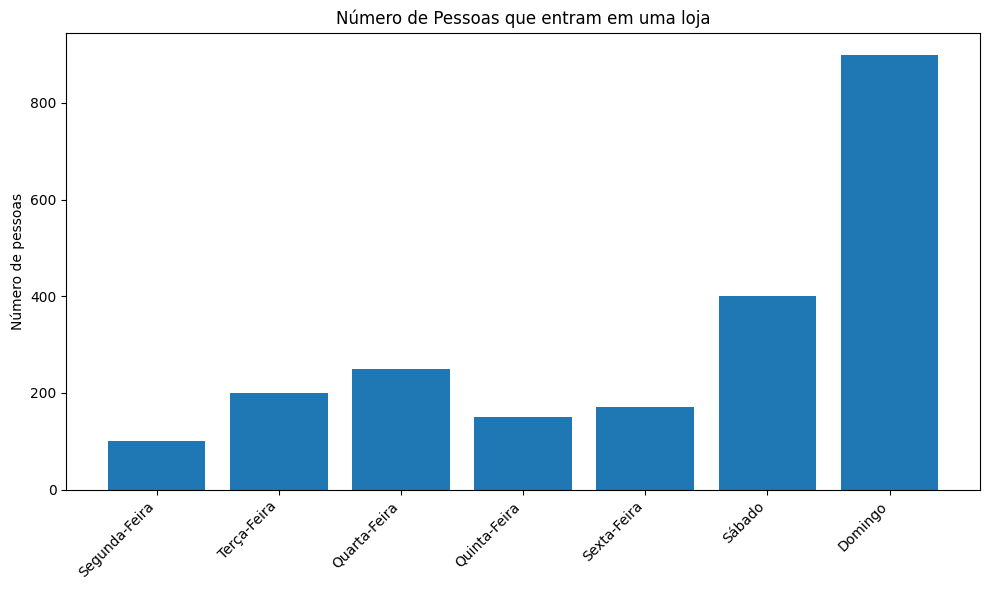
\includegraphics[scale=.6]{figuras/colunas}
\end{figure}

\inic Apresentaremos agora algumas formas de representação de amostras tento em vista a ordem de tabulação de dados. Diremos que os dados estarão organizados em ``Rol" se estes estiverem em ordem crescente ou decrescente. Em geral, um banco de dados $X =\{x_1,x_2, \cdots,x_n\}$ será representado como:

\begin{equation*}
    \begin{cases}
    x_{(1)}:\,\, \text{menor elemento da amostra};\\
    x_{(2)}:\,\,\text{2º menor elemento da amostra};\\
    \vdots\\
    x_{(n)}: \,\,\text{maior elemento da amostra.}\\
    \end{cases}
\end{equation*}
\inic Chamaremos de \textit{Amplitude} (h) o a diferença entre o maior e menor valor observado na amostra, isto é, $h = x_{(n)} - x_{(1)}$. Os gráfico apropriado para representamos dados em ordem crescente é o chamado \textit{gráfico de barras}, que é mostrado na Figura \ref{barras}

\begin{figure}[H]
    \label{barras}
	\centering
	\caption{Gráfico de Barras}
	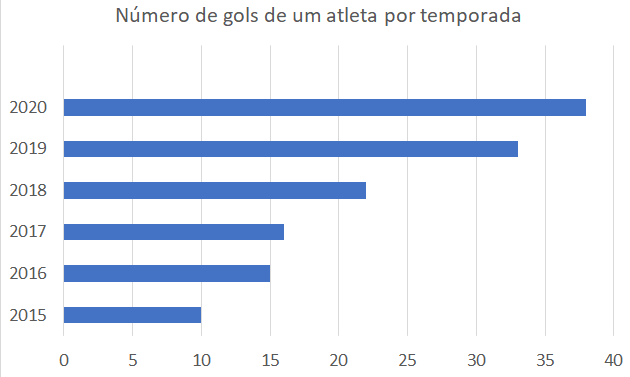
\includegraphics[scale=.6]{figuras/barras}
\end{figure}

\inic Note que a barras estão sempre na ordem crescente de quantidade de dados, o que caracteriza e diferença este gráfico.

\begin{defin}
Seja um banco de dados $X = \{x_1,x_2,x_3, \cdots, x_n\}$ chamamos de frequência absoluta ($f_i$) o número de vezes que o dado $x_i$ aparece na amostra.
\end{defin}
Vale salientar que cada $x_i$ pode ter diferentes significados, podendo até mesmo representar intervalos da reta (classes). O arranjo de valores com suas respectivas frequências é denominado \textit{Distribuição de Frequência}.

\noindent \exemplo
\begin{enumerate}
    \item[(i)] Em um hospital há cinco setores, a Tabela \ref{exemplo1} mostra a os leitos ocupados por setor:
\begin{table}[H]
    \caption{Generalização do crescimento simples}
    \label{exemplo1}
    \centering
    \begin{tabular}{cc}
    \hline
    Setor & $f_i$ \\
    \hline
    1 & 30 \\
    2 & 10 \\
    3 & 25 \\
    4 & 32 \\
    \hline
    \end{tabular}
\end{table}
\end{enumerate}
\inic Em geral tabelamos o par $(x_i, f_i)$ para melhor entendimento do leitor.
\section{Intervalos de Classe}
Agrupamos dados contínuos em intervalos de classes, que são definidos pelos símbolos ``$\vdash$" aberto a direita e fechado a esquerda e são distribuídos conforme a Tabela \ref{classes} 
	\begin{table}[H]
        \centering
        \caption{Intervalos de Classe}
        \label{classes}
		    \begin{tabular}{cc}
		    \hline
		    $\mathnormal{x_i}$ & $\mathnormal{f_i}$\\
		    \hline
		    35 $\vdash$ 45 & 5\\
		    45 $\vdash$ 55 & 12\\
		    55 $\vdash$ 65 & 18\\
	    	65 $\vdash$ 75 & 14\\
	    	75 $\vdash$ 85 & 6\\
	    	85 $\vdash \hspace{-0.2 cm }\dashv$ 95 & 3\\
		    \hline
		\end{tabular}
	\end{table}
	
Sendo $\vdash \hspace{-0.2 cm }\dashv$ intervalo fechado à direita e à esquerda. Os "$\mathnormal{f_i}$'s" \, representam a quantidade de valores que estão no intervalo indicado por $\mathnormal{x_i}$. a forma gráfica de representar intervalos de classe é dada pelos \textit{histogramas} que são gráficos conforme a Figura \ref{histo}
    
    \begin{figure}[H]
    \label{histo}
		\centering
		\caption{Histograma da Tabela \ref{classes}}
		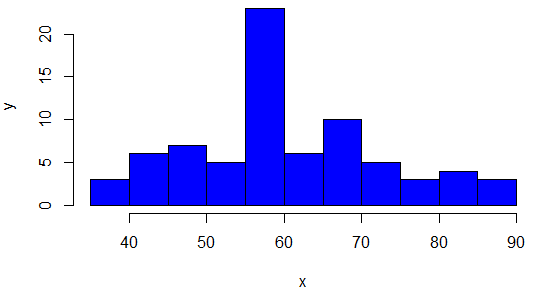
\includegraphics[scale=1]{figuras/histo}
	\end{figure}
	
\inic Posteriormente indicaremos o histograma como gráfico mais apropriado para entendermos como uma distribuição de probabilidade se comporta.

\section{Tabelas Estatísticas}
\inic Uma tabela estatística deve apresentar os seguintes elementos básicos:

\begin{enumerate}
	\item[(i)] Cabeçalho;
	\item[(ii)] Corpo, colunas e subcolunas da tabela;
	\item[(iii)] Rodapé, reservado para informações importantes da tabela.
\end{enumerate}
\inic Um bom cabeçalho deve responder os seguintes questionamentos:
\begin{enumerate}
	\item[(i)] O que está sendo representado?
	\item[(ii)] Onde ocorreu? 
	\item[(iii)] Quando ocorreu?
\end{enumerate}

\subsection{Série Temporal}
\inic Uma série de dados observado segundo a época de ocorrência:

\begin{table}[H]
    \centering
	\caption{Série temporal}
    \label{temporal}
	\begin{tabular}{cc}
		\hline
		Ano & Vendas\\
		\hline
		1970 & 2108 \\
		1971 & 1542 \\
		1972 & 3225 \\
    	1973 & 4788 \\
    	1974 & 1245 \\
		1975 & 3569 \\
		1976 & 4785 \\
		\hline
		\end{tabular}
		\\
	    Fonte: \cite{da1981curso}
	\end{table}
\subsection{Série Geográfica}
\inic É uma série estatística em que os dados são agrupados segundo modalidade de ocorrências 
\begin{table}[H]
    \centering
    \caption{Série Geográfica}
    \label{tab:my_label}
    \begin{tabular}{cc}
		\hline
		Regiões & Número\\
		\hline
		Norte & 7025 \\
		Nordeste & 107783 \\
		Sudeste & 218207 \\
		Sul & 15776 \\
		Centro-Oeste & 5243 \\
		\hline
	\end{tabular}
\end{table}
\subsection{Série Específica}
\inic É uma série estatística em que os dados são agrupados segundo modalidade de ocorrências, temos como exemplo a Tabela 
	\begin{center}
		\textbf{Matrículas no Ensino de Técnico Grau} \\
		\begin{tabular}{cc}
			\hline
			Áreas & Matrículas\\
			\hline
			Biologia & 32109 \\
			Agrárias & 107783 \\
			Letras & 2458 \\
			Artes & 3254 \\
			Histórias & 2451\\
			\hline
		\end{tabular}
		\\
		\textbf{Fonte}: \cite{da1981curso}
	\end{center}
\inic Note que a tabela representa a quantidade de indivíduos que obedecem a uma determinada categoria.
\section{Medidas de Tendência Central e de Posição}
\inic Buscamos estabelecer medidas para analisar os dados, buscamos valores que de fato consigam explicar a tendência e comportamento dos dados, apresentaremos nessa seção algumas medidas de tendência central e de posição que buscam explicar como os dados se comportam mediante a um determinado fenômeno, para explanar melhor definiremos o conceito de \textit{Média Arimética} de um banco de dados de tamanho $n$ dado por $X = \{x_1,x_2,x_3,\cdots,x_n\}$, de fato definimos média aritmética, denotada por $\overline{x}$ a expressão

\begin{equation}
\label{media}
    \overline{x} = \frac{\displaystyle\sum_{i=1}^{n}x_i}{n} = \frac{x_1+ x_2 + x_3 + \cdots + x_n}{n}
\end{equation}

\noindent \exemplo
\begin{enumerate}
    \item[(i)] Seja o banco de dados $X = \{2,2,2,2,3,4,5,5,10\}$ determine a sua média aritmética. Basta usar a expressão (\ref{media}) logo
    \begin{align*}
        \overline{x} = \frac{2+2+2+2+3+4+5+5+10+10}{10} = 4
    \end{align*}
        
    \item [(ii)] Um professor, para fazer a sua auto crítica, resolve analisar as médias das notas das turmas que estão dispostas na Tabela \ref{exemplomedia}
    
    \begin{table}[H]
        \caption{Média das turmas}
        \centering
        \label{exemplomedia}
        \begin{tabular}{cc}
        \hline
        Turma & Notas \\
        \hline
        A & 5,75 \\
        B & 7,0 \\
        C & 3,5 \\
        D & 9,1 \\
        \hline
    \end{tabular}
\end{table}
\inic Observe que, apenas pela média das notas podemos verificar se a a turma por completo está tendo aprendizado, isto é, a Turma C tem muito mais dificuldade que a Turma D devido as notas. Vale salientar que o resultado é dado ``em média", ou seja, não necessariamente algum aluno da turma A tirou a nota 5,75 e também pode ter ocorrido notas 10,0 e/ou zero. Em suma podemos representar a representação geométrica em forma de conjunto, é dada pela Figura \ref{mediaintgeo}

\begin{figure}[H]
    \label{mediaintgeo}
	\centering
	\caption{Média no banco de dados}
	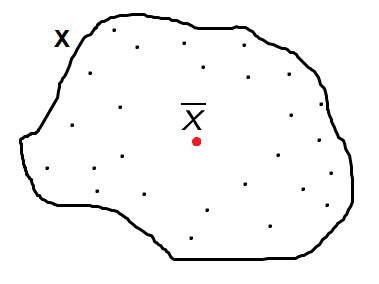
\includegraphics[scale=.8]{figuras/medida}
\end{figure}
\end{enumerate}
\inic Observe que nenhum dos dados são exatamente a média, porém todos estão em torno da média. Dizemos também, que uma média é bem representativa se todos os números desse banco de dados forem substituídos por $\overline{x}$, uma certa peculiaridade, por exemplo, soma ou produto dos números, será mantida. 

\subsection{Média para dados tabelados}
Como já vimos, dados tabelados são colocados em distribuição de frequência, considere o banco de dados $X_f=\{(x_1,f_i);(x_2,f_2);(x_3,f_3) \cdots, (x_n,f_n)\}$, sendo cada $x_i$ com sua respectiva frequência, logo a média aritmética é dada por

\begin{equation}
\label{tabelados}
    \overline{x} = \dfrac{\displaystyle\sum_{i=1}^{n}x_if_i}{\displaystyle\sum_{i=1}^nf_i} = \dfrac{x_1f_1 + x_2f_2 + x_3f_3 + \cdots + x_nf_n}{f_1 + f_2 + f_3 + \cdots + f_n},
\end{equation}
isto é, multiplicamos cada valor pela sua frequência e dividir pelo total de dados, ou seja, a soma das frequências.

\noindent \exemplo
\begin{enumerate}
    \item [(i)] Dada as distribuição de frequência, calcule a média aritmética
    \begin{table}[H]
        \caption{Distribuição de frequência }
        \centering
        \label{distri1}
        \begin{tabular}{cc}
        \hline
        $x_i$ & $f_i$ \\
        \hline
        2 & 10 \\
        3 & 5 \\
        4 & 12 \\
        6 & 11 \\
        \hline
    \end{tabular}
\end{table}
\inic Podemos fazer de duas formas, esteticamente falando, esse cálculo uma é usar diretamente a expressão \ref{tabelados}, que nos dá
\begin{align*}
    \overline{x} = \dfrac{2.10 + 3.5 + 4.12+6.11}{10+5+12+11} = 3,9210,
\end{align*}
a outra forma de realizar esta operação é criando novas colunas na Tabela \ref{distri1}, logo
\begin{table}[H]
        \centering
        \label{distri2}
        \begin{tabular}{ccc}
        \hline
        $x_i$ & $f_i$ & $x_if_i$ \\
        \hline
        2 & 10 & 20\\
        3 & 5 & 15\\
        4 & 12 & 48\\
        6 & 11 & 66\\
        \hline
        $\Sigma$ & 38 & 149
    \end{tabular}
\end{table}
\inic Basta agora dividirmos $149/38 = 3,9210$ .É importante frisar que, quando temos valores muitos diferentes dos demais, chamados valores aberrantes ou extremos, que não devemos utilizar a média aritmética para representa-los, pois esta é fortemente influenciada. Note pelo exemplo (ii)
\item [(ii)] Dada as distribuição de frequência, calcule a média aritmética
    \begin{table}[H]
        \caption{Distribuição de frequência }
        \centering
        \label{distri2}
        \begin{tabular}{cc}
        \hline
        $x_i$ & $f_i$ \\
        \hline
        2 & 10 \\
        3 & 5 \\
        4 & 12 \\
        6 & 11 \\
        1000 & 1\\
        \hline
    \end{tabular}
\end{table}
\begin{align*}
    \overline{x} = \dfrac{2.10 + 3.5 + 4.12+6.11+ 1000.1}{10+5+12+11+1} = 29,46,
\end{align*}
perceba que a média $29,46$ não representa bem os dados, pois a maioria destes estão abaixo de $10$ por exemplo.
\end{enumerate}
\subsection{Média ponderada}
Sejam os número reais $\{\omega_1, \omega_2,\omega_3,\cdots, \omega_n$\}. Quando queremos dar importância a mais para um tipo de dado do banco utilizamos a média ponderada, e chamamos cada $\omega_i$ de peso. definimos média ponderada por
\begin{equation}
    \label{peso}
    \overline{x} = \dfrac{\displaystyle\sum_{i=1}^{n}x_i\omega_i}{\displaystyle\sum_{i=1}^n\omega_i} = \dfrac{x_1\omega_1 + x_2\omega_2 + x_3\omega_3 + \dots + x_n\omega_n}{\omega_1 + \omega_2 + \omega_3 + \cdots + p_n},
\end{equation}
note que a média ponderada é uma generalização da média para dados tabelados, tento em vista que cada $f_i \in \mathbb{N}$ e cada $\omega_i \in \mathbb{R}$ sendo $\mathbb{N}\subset \mathbb{R}$.

\noindent \exemplo
\begin{enumerate}
    \item [(i)] Uma empresa de comunicação conta com 4 categorias de funcionários: Recepcionistas, Motoristas, Telemarketing e Diretoria. Os funcionários da primeira categoria recebem R\$ 950,35 mensalmente, segunda ganha R\$1.100,35 a terceira R\$ 1.111,21 enquanto os da quarta recebem R\$ 9501,53. Sabendo que essa empresa possui 63 funcionários no setor de telemarketing, 5 diretores, 4 motoristas e 12 recepcionistas, qual o salário médio pago por essa empresa? 
    \begin{align*}
        \overline{x} &= \dfrac{\displaystyle\sum_{i=1}^{4}x_i\omega_i}{\displaystyle\sum_{i=1}^4\omega_i} = \dfrac{x_1\omega_1 + x_2\omega_2 + x_3\omega_3+ x_4\omega_4}{\omega_1 + \omega_2 + \omega_3 + \omega_4}\\
        &= \dfrac{12.950,35 + 4.1100,35 + 63.1111,21 + 4.9501,53}{5 + 4 + 12 + 63} = 1474,02,
    \end{align*}
    \item[(ii)] (UNIUBE MG/2014) Um aluno deve atingir 70 pontos para ser aprovado. Esse total de pontos é resultado de uma média ponderada de 3 notas, $N_1$, $N_2$ e $N_3$, cujos pesos são, respectivamente, 1, 2, 2. As suas notas, $N_1$ e $N_2$, são, respectivamente, em um total de 100 pontos distribuídos em cada uma, 50 e 65. Para ser aprovado qual a nota $N_3$ numa escalade 0 a 100? 
    
    Neste problema temos a média o qual queremos atingir $\overline{x}=70$, e nos sobrará apenas os valor de $N_3$ logo, temos
    \begin{align*}
        70 &= \dfrac{1.50+2.65+2.N_3}{5}\\
        350 &= 2N_3 + 180 \\
        N_3&=85
    \end{align*}
\end{enumerate}

\subsection{Média em Intervalos de Classe}
\inic Para o cálculo da média quando os dados são contínuos, isto é, estão tabulados em intervalos de classe, basta definimos o ponto $p_i$ que é o ponto médio do intervalo da classe ($\ell_i$ = limite inferior do intervalo, $\ell_s$ = limite superior do intervalo) de calcularmos uma média para dado tabulados, levando em consideração o centro do intervalo, ou seja, sejam $n$ intervalos de classe, cada um com frequência $f_i$, então
\begin{equation}
    \overline{x} = \dfrac{\sum^{n}_{i=1}x_ip_i}{\sum^{n}_{i=1}p_i}
\end{equation}
Com $p_i = \dfrac{\ell_i + \ell_s}{2}$. 
\subsection{Média Geral}
\inic Sejam $\overline{x}_1, \overline{x}_2, \overline{x}_3, \cdots, \overline{x}_k$ as médias de $k$ séries de dados, com $n_1,n_2,n_3, \cdots, n_k$ o número de termos de cada série. Chamamos média geral, denotada por $\overline{x}^{(g)}$ a expressão
\begin{equation}
    \overline{x}^{(g)} =  \frac{\displaystyle\sum_{i=1}^{n}\overline{x}_in_i}{\displaystyle\sum_{i=1}^{n}n_i} = \frac{n_1\overline{x}_1 + n_2\overline{x}_2 + n_3\overline{x}_3 + \cdots + n_k\overline{x}_k}{n_1 + n_2 + n_3 +  \cdots, + n_k},
\end{equation}
em suma, para calcular uma média geral, você precisa ter $k$ bancos de dados, suas médias e seus respectivos tamanhos. Basicamente, a média geral é também uma média ponderada usando como pesos a quantidade de indivíduos do banco de dados.

\begin{figure}[H]
    \label{mediaintgeo}
	\centering
	\caption{Média Geral}
	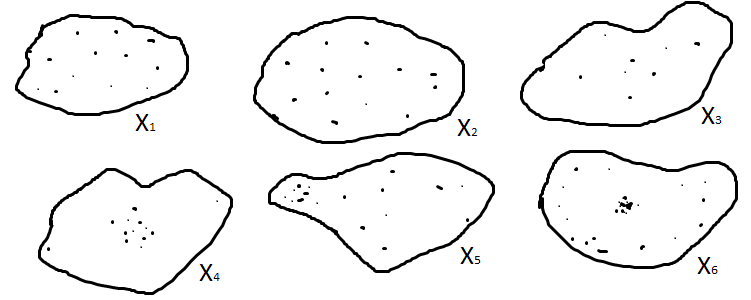
\includegraphics[scale=.8]{figuras/banco6}
\end{figure}

\noindent \exemplo
\begin{enumerate}
    \item [(i)] Considere o banco de dados com médias $\overline{x} = 10$ e $\overline{y} = 11,42$ sendo $\sum_{i=1}^{n}x_i=50$ e $\sum_{j=1}^{m}y_i=80$, calcule o número de elementos de cada população e a média geral.
    
    \inic Para calcular a média geral, basta determinarmos quantos indivíduos existem em cada população, de fato
    \begin{align*}
        \overline{x} = \frac{\sum_{i=1}^{n}x_i}{n_x} \Rightarrow n_x = \frac{\sum_{i=1}^{n}x_i}{\overline{x}} \Rightarrow n_x = \frac{50}{10} = 5\\
         n_y = \frac{\sum_{j=1}^{m}y_j}{\overline{y}} \Rightarrow n_y = \frac{80}{11,42} \approx 7 
    \end{align*}
    Agora basta calculamos a média geral, temos
    \begin{align*}
        \overline{x}^{(g)} = \frac{\overline{x}n_x + \overline{y}n_y}{n_x+n_y} = \frac{10.5+11,42.7}{5+7} = \frac{20}{3}
    \end{align*}
    
    \item[(ii)] Em uma empresa a média de idade das mulheres é $\overline{M} = 28$ e dos homens é $\overline{H} = 32$, sabe-se que somando as idades de todos os homens temos $544$, e se somarmos a idade das mulheres temos $644$. Determine a média de idade dos funcionários dessa empresa.
    
    \inic Temos um problema parecido com o anterior, com a diferença o contexto que não pede de maneira explícita o cálculo da média geral, de fato, vamos calcular primeiramente quantos homens e quantas mulheres há nesta empresa.  
    \begin{align*}
    n_M &= \frac{644}{28} = 23, \\
    n_H &= \frac{544}{32} = 17.
    \end{align*}
    \inic Agora, calculamos a média geral, logo
    \begin{equation*}
        \overline{x}^{(g)} = \frac{\overline{H}n_H + \overline{M}n_M}{n_H+n_M} = \frac{32.17 + 28.23}{23+17} = 29,7.
    \end{equation*}
    
\end{enumerate}

\subsection{Outras Médias}
\subsubsection{Média Geométrica}
Considere novamente o banco de dados $X$ associados ao conjunto de frequências $F$, a média geométrica $\overline{x}_g$ é definida por

\begin{equation}
    \overline{x}_g = \sqrt[n]{\prod_{i=1}^nx_i} = \sqrt[n]{x_1x_2x_3\cdots x_n}.
\end{equation}
\inic A média geométrica possui aplicações em diversas áreas da ciência, uma das aplicações mais usuais é no mercado financeiro, ao invés de calcularmos a média arimética, usamos a geométrica para cálculos de taxas médias.
Seja o banco de dados $\mathnormal{X}= \{\mathnormal{x}_1,\mathnormal{x}_2,\mathnormal{x}_3,\cdots, \mathnormal{x_n}\}$ com $\mathnormal{n}$ elementos, e suas respectivas frequências $\mathnormal{F} = \{\mathnormal{f}_1,\mathnormal{f}_2,\cdots,\mathnormal{f_n}\}$, assim calculamos:


\begin{equation}
	\overline{\mathnormal{x}}_{\mathnormal{g}} = \sqrt[\mathnormal{n}]{\mathnormal{x}_1^{\mathnormal{f}_1}\mathnormal{x}_2^{\mathnormal{f}_2}\mathnormal{x}_3^{\mathnormal{f}_3}\cdots \mathnormal{x_n}^{\mathnormal{f_n}}}
\end{equation}
em alguns momentos será necessário o cálculo de $\log \mathnormal{\overline{x}_g}$ pela expressão:
\begin{equation*}
	\log \overline{x}_g = \dfrac{\displaystyle\sum_{i=1}^{n} f_i \log x_i}{n} = \frac{f_1 \log x_1 + \cdots + f_n \log x_n}{n}
\end{equation*}

\noindent \exemplo
\begin{enumerate}
	\item[(i)] Calcule a média geométrica dos dados abaixo:
		\begin{enumerate}
			\item[(a)] 3 - 6 - 12 - 24 - 48;
			\item[(b)] \begin{tabular}{ll}
				\hline
				$\mathnormal{x_i}$ & $\mathnormal{f_i}$\\
				\hline
				1 & 8 \\
				2 & 6 \\
				3 & 5 \\
				5 & 3 \\
				\hline
			\end{tabular}
		\end{enumerate}
		%\item[(ii)]
	\end{enumerate}

\subsubsection{Média Harmônica}
Os comentários e exemplos aqui citados, foram retirados de \cite{hariki1996media}.

Um número $\overline{x}_H$ é a média harmônica de um conjunto de banco de dados $X$ se 
\begin{align}
    \label{harmonica}
    \frac{1}{x_1} + \frac{1}{x_2} + \frac{1}{x_3} + \cdots + \frac{1}{x_n} &= \underbrace{\frac{1}{\overline{x}_H} + \frac{1}{\overline{x}_H} + \frac{1}{\overline{x}_H} + \cdots + \frac{1}{\overline{x}_H}}_{n},\\
    \label{harmonica2}
    \frac{1}{x_1} + \frac{1}{x_2} + \frac{1}{x_3} + \cdots + \frac{1}{x_n} &= \frac{n}{\overline{x}_H},\\ 
    \label{harmonica3}
    \overline{x}_H &= \frac{n}{\frac{1}{x_1} + \frac{1}{x_2} + \frac{1}{x_3} + \cdots + \frac{1}{x_n}}
\end{align}
Para dados agrupados temos 
\begin{equation}
    \overline{x}_H = \frac{f_1 + f_2 + f_3 + \cdots + f_n}{\frac{f_1}{x_1} + \frac{f_2}{x_2} + \frac{f_3}{x_3} + \cdots + \frac{f_n}{x_n}},
\end{equation}
a ideia de média harmônica aparece quanto pretendemos calcular uma média entre razões de grandezas sendo a grandeza do numerador é a mesma dentro do problema específico. 

\noindent \exemplo
\begin{enumerate}
    \item [(i)] Determine a média harmônica entre 2, 5, 8.
    Basta aplicarmos a expressão \ref{harmonica3}, para $n=3$, logo
    \begin{align*}
        \overline{x}_H = \frac{3}{\frac{1}{2} + \frac{1}{5} + \frac{1}{8}} = 3,64
    \end{align*}
    \item[(ii)] Um motorista vai de Recife a Caruaru com uma velocidade média de $80 km/h$. Chegando lá, retorna, utilizando o mesmo percurso, para o local onde partiu em Recife, com velocidade de média de $100 km/h$. Qual a velocidade média do percurso? 
    
    \inic Note que no problema queremos a média da razão \textit{deslocamento}/\textit{tempo}, na qual o deslocamento é o mesmo para as duas razões. Então tome $d$ deslocamento, $t_i$ o tempo de ida, $t_v$ o tempo de volta e $V$ a velocidade média, logo
    \begin{align*}
        V&= \frac{2d}{t_i + t_v}\Rightarrow t_i + t_v = \frac{2d}{V},\,\, \text{como}\,\, t_i = \frac{d}{80}\,\, \text{e}\,\, t_v = \frac{d}{100}\\
        \frac{2}{V} &= \frac{1}{80} + \frac{1}{100} \Rightarrow V \approx 88,9 km/h
    \end{align*}
    \item[(iii)] Um grande tanque possui três torneiras. A torneira A enche o tanque em 4h, a B, em 3h e a C em 6h. Deseja-se substituí-las por três torneiras idênticas, de modo que essas três novas ligadas simultaneamente encham o tanque no mesmo tempo que as torneiras A, B e C ligadas juntas. Quanto tempo será necessário par apenas umas dessas novas torneiras encher o tanque? 
    
    \inic Aqui tomaremos o tempo unitário, isto é, em 1h vemos que a torneira $A$ enche $1/4$ do tanque, a $B,\,\,1/3$ e a $C,\,\,1/6$. Digamos que as torneiras novas encham, sozinhas, cada uma o tanque em $T$ horas. Logo, cada uma, em 1h encherá $1/T$ do tanque. Portanto, em uma hora a fração do tanque que estará cheia será: 
    \begin{align*}
        \frac{3}{T} &= \frac{1}{4} + \frac{1}{3} + \frac{1}{6},\\
        T&=4.
    \end{align*}
\end{enumerate}

\section{Medidas de Posição}
\subsection{Mediana}

\begin{defin}
Sejam um banco de dados $X = \{x_1,x_2,x_3,\cdots, x_n\}$, definimos mediana, denotado por $\Tilde{x}$, o valor numérico que divide a série de dados em duas partes de tamanhos iguais.
\end{defin}
Geometricamente, em uma dimensão, podemos representar a medida por

\begin{figure}[H]
	\centering
	\caption{Interpretação geométrica da Mediana}
	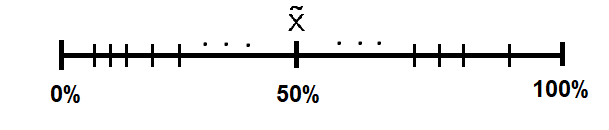
\includegraphics[scale=.9]{figuras/mediana.png}
\end{figure}
Importante frisar que a mediana é uma medida que não é afetada por valores extremos. Para determinar posição da mediana, em dados discretos, temos dois casos:
	\begin{equation}
	\label{medianadis}
		\Tilde{x} = \begin{cases}
		\mathnormal{x}_{\left(\frac{\mathnormal{n}+1}{2}\right)}, \, \text{se}\,\, \mathnormal{n}\,\,\text{é impar}\\
		\\
		\dfrac{\mathnormal{x}_{\left(\frac{\mathnormal{n}}{2}\right)}+\mathnormal{x}_{\left(\frac{\mathnormal{n}}{2}+1\right)}}{2}, \,\,\text{se}\,\, \mathnormal{n}\,\,\text{é par}
		\end{cases}
	\end{equation}	
para calcular a mediana para dados contínuos, ou seja, tabulados em intervalos de classe temos os seguintes passos

\begin{enumerate}
    \item[(i)] Calcula-se a ordem $n/2$, sendo $N = \sum f_i$;
    \item[(ii)] Use a $f_{ac}$ para identificar a classe mediana;
    \item[(iii)] Utiliza-se a fórmula:
    \begin{equation}
    \label{medianacont}
    \tilde{x} = \ell_{\tilde{x}} + \frac{\left(\dfrac{N}{2}-\sum f_i\right)h}{f_{\tilde{x}}}
    \end{equation}
\end{enumerate}
sendo
\begin{itemize}
     \item $\ell_{\tilde{x}}$: limite inferior da classe mediana;
     \item $N$: número de elementos;
     \item $\sum f$: soma das frequências anteriores à classe mediana;
     \item $h$: amplitude da classe mediana;
     \item $f_{\tilde{x}}$: frequência da classe mediana.
\end{itemize}

\noindent \exemplo
\begin{enumerate}
    \item[(i)] Calcule a mediana dos dados abaixo:
    \begin{enumerate}
        \item[(a)] 8 - 5 - 8 - 10 - 8 - 9 - 10 - 9 - 12 - 13 - 20 - 30 - 40;
        \item[(b)] 
        \begin{center}
        \begin{tabular}{cc}
            \hline
            $x_i$ & $f_i$ \\
            \hline
            2  & 4  \\
            4  & 8  \\
            8  & 16 \\
            16 & 32 \\
            32 & 64 \\
            \hline
        \end{tabular}
        \end{center}

        \item[(c)] 
        \begin{center}
        \begin{tabular}{cc}
            \hline
            $x_i$ (classe) & $f_i$ \\
            \hline
            35 $\vdash$ 45 & 5  \\
            45 $\vdash$ 55 & 12 \\
            55 $\vdash$ 65 & 18 \\
            65 $\vdash$ 75 & 14 \\
            75 $\vdash$ 85 & 6  \\
            85 $\vdash\hspace{-0.2cm}\dashv$ 95 & 3 \\
            \hline
        \end{tabular}
        \end{center}
    \end{enumerate}
\end{enumerate}

\inic O item (a) basta colocarmos os dados em ordem crescente identificarmos a paridade de $n$, logo\\

\begin{center}
 5 - 8 - 8 - 8 - 8 - 9 - 9 - 9 - 10 - 10 - 12 - 13 - 20 - 30 - 40   
\end{center}
 como temos $ n = 15$, logo usando a expressão (\ref{medianadis}), temos
 $$
 \Tilde{x} = x_{\left(\frac{n+1}{2}\right)} = x_{\left(\frac{15+1}{2}\right)} = x_{(8)}
 $$
isto é, a mediana será o elemento $x_{(8)} = 9$.

\inic Para o item (b), basta identificarmos a também onde se localiza $\sum f_i/2$, isto é, $\sum f_i/2 = 124/2 = 62$ e agora construimos a coluna de frequências acumuladas, logo

\begin{table}[H]
    \centering
    \begin{tabular}{ccc}
	\hline
	$x_i$ & $f_i$ & $f_{ac}$\\
	\hline
	2 & 4 & 4\\
	4 & 8 & 12\\
	8 & 16 & 28\\
	16 & 32 & 60\\
	32 & 64 & 124\\
	\hline
    \end{tabular}
\end{table}
\inic Logo a mediana será o dado cuja frequência ultrapassou $\sum f_i/2 = 62$, isto é, $\Tilde{x} = 32$.

\inic Para o item (c) usaremos (\ref{medianacont}) e seguiremos os passos dados, assim 
\begin{table}[H]
    \centering
    \begin{tabular}{ccc}
	    \hline
	    $x_i$ & $f_i$ & $f_{ac}$\\
	    \hline
	    35 $\vdash$ 45 & 5 & 5\\
        45 $\vdash$ 55 & 12 & 17\\
	    55 $\vdash$ 65 & 18 & 35\\
        65 $\vdash$ 75 & 14 & 49\\
	    75 $\vdash$ 85 & 6 & 55\\
	    85 $\vdash \hspace{-0.2 cm }\dashv$ 95 & 3 & 58\\
	    \hline
    \end{tabular}
\end{table}

\inic Logo pelo critério do item (b)  definimos a classe que contém a mediana como sendo $55 \vdash 65$ e assim

\begin{equation*}
    \begin{cases}   
        \ell_{\Tilde{x}} = 55\\
        N/2 = 29\\
        \sum f_i = 17\\
        h = 65-55 = 10\\
        f_{\Tilde{x}} = 18,
    \end{cases}
\end{equation*}
Agora basta substituir em (\ref{medianacont}), temos

\begin{align*}
    \tilde{x} &= \ell_{\tilde{x}} + \frac{\left(\dfrac{N}{2} - \sum f_i \right) h}{f_{\tilde{x}}} \\
    &= 55 + \frac{(29 - 17) \cdot 10}{18} \approx 61{,}67
\end{align*}



\subsection{Quartis}
\inic Seja o banco de dados $X$ organizados em rol, definem-se \textit{quartis} os valores da distribuição que dividem o banco de dados em quatro partes iguais, isto é:

	\begin{figure}[H]
		\centering
		\caption{Forma geométrica dos quartis em uma dimensão}
		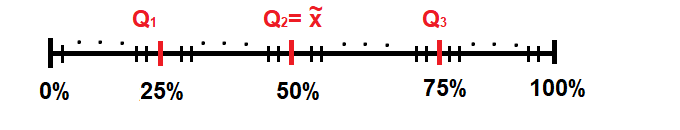
\includegraphics[scale=.8]{figuras/quartis.png}
	\end{figure}
	
	Como $Q_2 = \tilde{x}$, para calcular $Q_1$ e $Q_3$, temos:
\begin{equation}
    \label{quartis}
    Q_i = \ell_{Q_i} + \dfrac{\left(\dfrac{in}{4} - \sum f_i \right) h}{f_{Q_i}}.
\end{equation}

\begin{itemize}
    \item $\ell_{Q_i}$: limite inferior da classe do quartil;
    \item $\sum f$: soma das frequências anteriores à classe do quartil;
    \item $h$: amplitude da classe do quartil;
    \item $f_{Q_i}$: frequência da classe do quartil.
\end{itemize}

\noindent \exemplo

\subsection{Decis}

\inic Agora $X$ será organizado em rol. Definem-se \textit{decis} os valores da distribuição que dividem o banco de dados em dez partes iguais, isto é:
\begin{figure}[H]
    \centering
    \caption{Interpretação geométrica dos Decis em uma dimensão}
    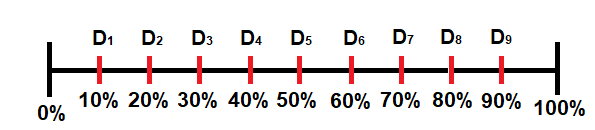
\includegraphics[scale=.7]{figuras/decil}
\end{figure}

Como $D_5 = \tilde{x}$, para calcular os demais, temos:
\begin{equation}
\label{decil}
D_i = \ell_{D_i} + \dfrac{\left(\dfrac{in}{10} - \sum f_i \right) h}{f_{D_i}}.
\end{equation}

\begin{itemize}
    \item $\ell_{D_i}$: limite inferior da classe do decil;
    \item $\sum f$: soma das frequências anteriores à classe do decil;
    \item $h$: amplitude
\end{itemize}

\subsection{Percentis}

\inic Seja $X$ organizado em rol. Definem-se \textit{percentis} os valores da distribuição que dividem o banco de dados em cem partes iguais, isto é:
\begin{figure}[H]
    \centering
    \caption{Interpretação geométrica dos Percentis em uma dimensão}
    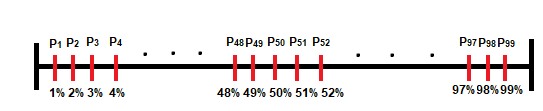
\includegraphics[scale=.7]{figuras/percentil}
\end{figure}

Como $P_{50} = \tilde{x}$, para calcular os demais, temos:
\begin{equation}
\label{percentil}
P_i = \ell_{P_i} + \dfrac{\left(\dfrac{in}{100} - \sum f_i \right) h}{f_{P_i}}.
\end{equation}

\begin{itemize}
    \item $\ell_{P_i}$: limite inferior da classe do percentil;
    \item $\sum f$: soma das frequências anteriores à classe do percentil;
    \item $h$: amplitude da classe do percentil;
    \item $f_{P_i}$
\end{itemize}
\inic O uso das fórmulas (\ref{quartis}), (\ref{decil}) e (\ref{percentil}) são todos semelhantes à (\ref{medianacont}), e podem ser perfeitamente aplicados a dados de exemplos anteriores.
Um esquema importante é o \textit{Esquema dos cinco números}. este procura estabelece as cinco principais estatísticas de ordem existentes que são: $x_{(1)}, x_{(n)}, Q_1, Q_3, Md$, isto é, mínimo, máximo, 25\% dos dados 50\% dos dados e 75\% dos dados. 


\subsection{Box plot}
\inic O \textit{box plot} é um gráfico que dá a ideia da posição, dispersão, assimetria, caudas e dados discrepantes, em geral é usado para analisar geometricamente as medidas de posição, temos

\begin{figure}[H]
	\centering
	\caption{Boxplot}
	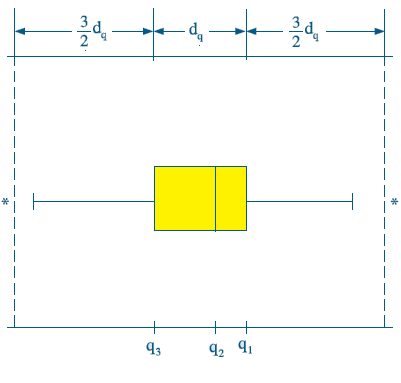
\includegraphics[scale=.6]{figuras/box.png}
	\begin{center}
	Fonte: \cite{morettin2017estatistica}
	\end{center}
\end{figure}

Para o cálculo dos elementos do \textit{Boxplot}, isto é, limites superior ($L_S$) e inferior ($L_I$) temos:
	\begin{equation}
		\begin{cases}
		    L_I = \max\{\min\{x_i\}, Q_1-1,5(Q_3-Q_1)\}\\
		    L_S = \min\{\max\{x_i\}, Q_1+1,5(Q_3-Q_1)\}
		\end{cases}
	\end{equation}

Para construir um \textbf{boxplot} no \textit{Rstudio} usaremos o comando \textbf{boxplot()}, que possui os seguintes argumentos básicos:
\begin{enumerate}
	\item[(i)] $x$ é o vetor de dados;
	\item[(ii)] ``main =" é o título do gráfico;
	\item[(iii)] ``xlab = "\, é o texto no eixo x;
	\item[(iv)] ``ylab = "\, é o texto no eixo y;
	\item[(v)] ``col ="\, é a cor do preenchimento da caixa;
	\item[(vi)] ``border ="\, cor da linha da borda da caixa; 
	\item[(vii)] ``horizontal ="\, se \textbf{TRUE} o gráfico ficará na horizontal, se \textbf{FALSE} ficará na vertical.
\end{enumerate}
\inic Outra importante ferramente é o comando ``fivenum(x, na.rm = TRUE)", que dá os 5 número representativos do boxplot.

\section{Moda ($M_o$)}
\inic Seja o banco de dados $\mathnormal{X}= \{\mathnormal{x}_1,\mathnormal{x}_2,\mathnormal{x}_3,\cdots, \mathnormal{x_n}\}$ com $\mathnormal{n}$ elementos, e suas respectivas frequências $\mathnormal{F}=\{\mathnormal{f}_1,\mathnormal{f}_2,\cdots,\mathnormal{f_n}\}$, definimos \textit{Moda} o valor de $\mathnormal{x_i}$ que possui maior frequência, isto é, seja o par $(\mathnormal{x_i,f_i})$ temos:
	\begin{equation*}
		Mo = \{\mathnormal{x_i} \in \mathbb{R}/ (\mathnormal{x_i}, max\{\mathnormal{f_1},\cdots,\mathnormal{f_n}\})\},
	\end{equation*}
para moda de dados discretos basta observamos a que possui maior $f_i$. Para dados em intervalos de classe temo a fórmula de Czuber, a qual seguiremos os seguinte passos
\begin{enumerate}
        \item[(i)] Identifica-se a classe modal;
		\item[(ii)] Usa-se a fórmula;
		\begin{equation}
		\label{Czuber}
		\mathnormal{Mo} = \ell_{Mo} + \frac{\mathnormal{\Delta}_1}{\mathnormal{\Delta}_1 + \mathnormal{\Delta}_2}\mathnormal{h},
		\end{equation}
	\end{enumerate}
	sendo:
	\begin{itemize}
		\item $\ell_{Mo}$: limite inferior da classe modal;
		\item $\mathnormal{\Delta}_1$: Diferença entre a frequência da classe modal e a imediatamente anterior;
		\item $\mathnormal{\Delta}_2$: Diferença entre a frequência da classe modal e a imediatamente posterior;
		\item $\mathnormal{h}$: amplitude da classe modal.
	\end{itemize}

\exemplo
\begin{enumerate}
    \item[(i)] Calcule a moda dos dados abaixo:
	\begin{enumerate}
	    \item[(a)] 8 - 5 - 8 - 10 - 8 - 9 - 10 - 9 - 12 -13 - 20 - 30 - 40;
		\item[(b)] \begin{tabular}{cc}
	    	\hline
			$\mathnormal{x_i}$ & $\mathnormal{f_i}$\\
			\hline
			2 & 4 \\
			4 & 8 \\
			8 & 16 \\
			16 & 32 \\
			32 & 64 \\
			\hline
		\end{tabular}
		\qquad \qquad (c) \begin{tabular}{cc}
			\hline
			$\mathnormal{x_i}$ & $\mathnormal{f_i}$\\
			\hline
			35 $\vdash$ 45 & 5\\
			45 $\vdash$ 55 & 12\\
			55 $\vdash$ 65 & 18\\
			65 $\vdash$ 75 & 14\\
			75 $\vdash$ 85 & 6\\
			85 $\vdash \hspace{-0.2 cm }\dashv$ 95 & 3\\
			\hline
		\end{tabular}
	\end{enumerate}
\end{enumerate}

\inic No Item (a) basta contarmos quais elementos aparecem mais, daí note que $M_o = 8$. Para o item (b) basta olharmos a coluna de frequências absolutas, note que a maior é do dado $x_i = 32$, logo $M_o = 32$. Para o item (c) aplicaremos os passos da fórmula de Czuber, logo \begin{equation*}
    \begin{cases}
        \mathtt{l}_{Mo} = 55\\
        \Delta_1 = 18-12 = 6\\
        \Delta_2 = 18- 14 = 4\\
        h = 10
    \end{cases}
\end{equation*}


\begin{align*}
    \mathnormal{Mo} &= \ell_{Mo} + \frac{\mathnormal{\Delta}_1}{\mathnormal{\Delta}_1 + \mathnormal{\Delta}_2}\mathnormal{h} = 55 + \frac{6}{6+4}10\\
    &= 61
\end{align*}
\inic Uma observação importante é que nem toda a série de dados possui apenas uma moda, poderíamos ter, por exemplo, um banco $X = \{2,2,3,3,4,5,6,7\}$, ou seja,um banco que possui duas modas, o que chamamos de \textit{série bimodal}, bem como temos com $3,4,\cdots, n$ modas, que são as séries $n$-modais. Se a série não possuir moda chamamos de \textit{Amodal}, por exemplo $Y = \{1,1,2,2,3,3,4,4,5,5\}$ 

\section{Medidas de Dispersão}
\inic São medidas que têm o objetivo de mensurar o afastamento dos dados de suas medidas de tendência central, em geral a média. Observe que na Figura há dois bancos de dados, que possuem a mesma média porém o dados não se comportam de maneira semelhante.

\begin{figure}[H]
	\centering
	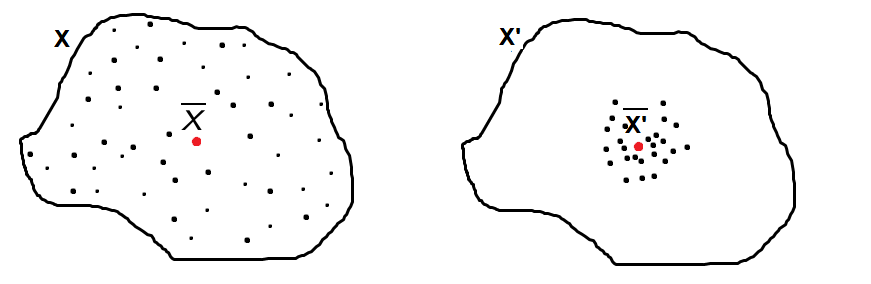
\includegraphics[scale=.65]{figuras/dispersao}
\end{figure}
\inic Note que em $X'$ os dados estão mais concentrados em torno da média, o que não ocorre com tanta evidência em $X$. Daremos agora um exemplo numérico da da situação explorada.

\noindent\exemplo\\
Sejam os bancos de dados $\mathnormal{X}=\{40,40,40,40,40,40,40\}$ e $\mathnormal{Y}=\{40, 60, 10,30,100,0,50,30\}$, note que $\mathnormal{\overline{x}} = \mathnormal{\overline{y}}= 40$, porém os bancos não possuem o mesmo comportamento, enquanto todos os valores de $X$ são exatamente iguais a média, os demais estão a uma certa distância não nula. Em estatística não podemos dizer que um banco de dados como $X$ e $Y$ são iguais, para diferenciar esses bancos de dados defini-se as \textit{medidas de dispersão}.

\subsection{Desvio}
\inic Seja o banco de dados $\mathnormal{X}$ com $\mathnormal{n}$ elementos e média $\mathnormal{\overline{x}}$ definimos desvio em relação ao dado $\mathnormal{x_i}$, denotado por $\mathnormal{D_i}$,  com $\mathnormal{i}=1,2,3,\cdots,\mathnormal{n}$ tal que:

\begin{equation}
	\mathnormal{D_i} = \mathnormal{x_i} - \mathnormal{\overline{x}}.	
\end{equation}
\inic Pelo fato termos indexado os desvios, cada dado terá o seu, de fato, observe o banco de dados do exemplo. 

\noindent \exemplo 

\begin{enumerate}
    \item [(i)] Determine os $D_i's$ do banco $X = \{5,2,3,4,5,5,6,10\}$.
    Primeiramente, vamos calcular a média deste banco de dados, temos 
    \begin{align*}
        \overline{x} = \dfrac{5 + 2 + 3 + 4 + 5 + 5 + 6 + 10}{8} = 5
    \end{align*}
\end{enumerate}
Agora, calcularemos os desvios dos dados, nesta ordem, $X = \{x_1 = 5,x_2 = 2,\cdots, x_8 = 10\}$ logo
\begin{equation*}
    \begin{cases}
    D_1 = x_1 - \overline{x} = 5 - 5 =0\\
    D_2 = x_2 - \overline{x} = 2 - 5 =-3\\
    D_3 = x_3 - \overline{x} = 3 - 5 =-2\\
    D_4 = x_4 - \overline{x} = 4 - 5 =-1\\
    D_5 = x_5 - \overline{x} = 5 - 5 =0\\
    D_6 = x_6 - \overline{x} = 5 - 5 =0\\
    D_7 = x_7 - \overline{x} = 6 - 5 =1\\
    D_8 = x_8 - \overline{x} = 10 - 5 =5
    \end{cases}
\end{equation*}
\begin{prop}
\label{desvios0}
A soma dos desvios é igual a zero.
\end{prop}

\begin{proof}
Considere o banco de dados $X = \{x_1,x_2,x_3,\cdots,x_n\}$ sendo que cada $x_i$ pode ser contínuo ou discreto. Então temos
\begin{align}
    \label{p1}
    D_i &= x_i - \overline{x}\\ 
    \label{p2}
    \sum_{i=1}^{n} D_i &= \sum_{i=1}^{n} (x_i - \overline{x})\\
    \label{p3}
      &= \sum_{i=1}^{n} x_i - n\overline{x}
\end{align}
mas pela definição de média temos $\overline{x} = \sum_{i=1}^{n} x_i/n \Rightarrow n\overline{x} = \sum_{i=1}^{n} x_i$ que substituindo em (\ref{p3}) concluímos a demonstração.
\end{proof}

\subsection{Desvio Médio}
No banco de dados $\mathnormal{X}$ com $\mathnormal{n}$ elementos e média $\overline{x}$, definimos \textit{desvio médio}, denotado por $\mathnormal{D_M}$ a expressão:
\begin{equation}
	D_M = \frac{\displaystyle \sum_{i=1}^{n}|x_i-\overline{x}|}{n},
	\end{equation}
para dados agrupados temos:
\begin{equation}
	D_M = \frac{\displaystyle \displaystyle \sum_{i=1}^{n} |x_i-\overline{x}|f_i}{n}
\end{equation}
Por exemplo, vamos calcular os desvio médio dos dados do exemplo da subseção de desvios, isto é, o conjunto $X = \{x_1 = 5,x_2 = 2,\cdots, x_8 = 10\}$, onde temos o conjunto de desvios $D = \{D_1 = 0, D_2 = -3, D_3 = -2, D_4 = -1, D_5 = 0, D_6 = 0, D_7 = 1, D_8 = 5\}$ agora calculando o desvio médio
\begin{align*}
    D_M &= \dfrac{\displaystyle \sum_{i=1}^{n} |D_i|}{n}\\
    &= \dfrac{|0| + |-3| + |-2| + |-1| + |0| + |0| + |1|+ |5|}{8}\\
    &= \dfrac{12}{8} = 1,5.
\end{align*}

\inic Isto é, em média os dados estão a uma distância de 1,5 da média. A definição de desvio médio é uma das soluções que foram encontradas para resolvermos o problema do cálculo de uma medida que represente a variação dos dados, tendo em vista o problema a Proposição \ref{desvios0}. Porém algumas propriedades de valor absoluto podem ser problema, por exemplo note que o valor absoluto não é uma função suave assim não pode-se derivar, para isso definiremos variância

\subsection{Variância}
\inic Outra forma de evitar que a soma dos desvio seja zero é considerando o quadrado da soma, assim definimos variância, denotada por $\sigma^2$ quando populacional e $s^2$ quando amostral, a expressão:
	\begin{equation}
	\label{var}
		\sigma^2 = \frac{\displaystyle \sum_{i=1}^{n} (x_i-\overline{x})^2}{n},
	\end{equation}
	para dados agrupados:
	\begin{equation}
	\label{varf}
		\sigma^2 = \frac{\displaystyle \sum_{i=1}^{n} (x_i-\overline{x})^2f_i}{\displaystyle\sum_{i=1}^{n} f_i}.
	\end{equation}

 \begin{defin}[Desvio Padrão]
    Definimos \textit{desvio padrão} por $\sigma = \sqrt{\sigma^2}$.
 \end{defin}
 
 \noindent \exemplo
 \begin{enumerate}
	\item[(i)] Nos dados abaixo, o desvio médio e o desvio padrão  de cada distribuição:
	\begin{enumerate}
		\item[(a)] 8 - 5 - 8 - 10 - 8 - 9;
		\item[(b)] \begin{tabular}{cc}
			\hline
			$x_i$ & $f_i$\\
			\hline
			5 & 2 \\
			6 & 3 \\
			8 & 5 \\
			9 & 32 \\
			11 & 64 \\
			\hline
		\end{tabular}
		\qquad \qquad \qquad (c) \begin{tabular}{cc}
			\hline
			$x_i$ & $f_i$\\
			\hline
			35 $\vdash$ 45 & 5\\
			45 $\vdash$ 55 & 12\\
			55 $\vdash$ 65 & 18\\
			65 $\vdash$ 75 & 14\\
			75 $\vdash$ 85 & 6\\
			85 $\vdash \hspace{-0.2 cm }\dashv$ 95 & 3\\
			\hline
		\end{tabular}
	\end{enumerate}
	Para solucionar o item (a) temos a aplicação da expressão (\ref{var}), para isso necessitamos da média, que será $\overline{x}=8$, logo o cálculo do desvio médio será
	\begin{align*}
	    D_M &= \frac{\displaystyle \sum_{i=1}^{6} |x_i-\overline{x}|}{n}\\
	     &= \dfrac{|x_1-\overline{x}| + |x_2-\overline{x}| + |x_3-\overline{x}| + |x_4-\overline{x}| + x_5-\overline{x}| + |x_6-\overline{x}|}{6}\\
	     &= \dfrac{|8-8| + |5-8| + |8-8| + |10-8| + |8-8| + |9-8|}{6}=\dfrac{6}{6}\\ 
	    &= 1
	\end{align*}
	e o desvio padrão
	\begin{align*}
	    \sigma^2 &= \frac{\displaystyle \sum_{i=1}^{6} (x_i-\overline{x})^2}{n}\\
	     &= \dfrac{(x_1-\overline{x})^2 + (x_2-\overline{x})^2 + (x_3-\overline{x})^2 + (x_4-\overline{x})^2 + (x_5-\overline{x})^2 + (x_6-\overline{x})^2}{6}\\
	     &= \dfrac{(8-8)^2 + (5-8)^2 + (8-8)^2 + (10-8)^2 + (8-8)^2 + (9-8)^2}{6}=\dfrac{14}{6}\\ 
	    &= 2,8,
	\end{align*}
	logo o desvio padrão será 
	\begin{equation*}
	    \sigma = \sqrt{\sigma^2} = \sqrt{2,8} = 1,6732
	\end{equation*}
\end{enumerate}
 No item (b) temos que $\overline{x} = 20$ e aplicaremos a expressão (\ref{varf}), logo
 \begin{align*}
	    \sigma^2 &= \frac{\displaystyle \sum_{i=1}^{5} (x_i-\overline{x})^2f_i}{\displaystyle\sum_{i=1}^{5}f_i}\\
	     &= \dfrac{(x_1-\overline{x})^2f_1 + (x_2-\overline{x})^2f_2 + (x_3-\overline{x})^2f_3 + (x_4-\overline{x})^2f_4 + (x_5-\overline{x})^2f_5}{f_1 + f_2 + f_3 + f_4 + f_5}\\
	     &= \dfrac{(5-20)^22 + (6-20)^23 + (8-20)^25 + (9-20)^232 + (11-20)^264}{106}=\dfrac{10814}{106}\\ 
	    &= 102,0188
	\end{align*}
\section{Assimetria e Curtose}
\subsection{Assimetria}
\inic Chamamos \textit{assimetria} o grau de afastamento de uma distribuição da unidade de simetria. Em uma distribuição simétrica tem-se a igualdade dos valores da média, mediana e moda, logo
\begin{figure}[H]
	\centering
	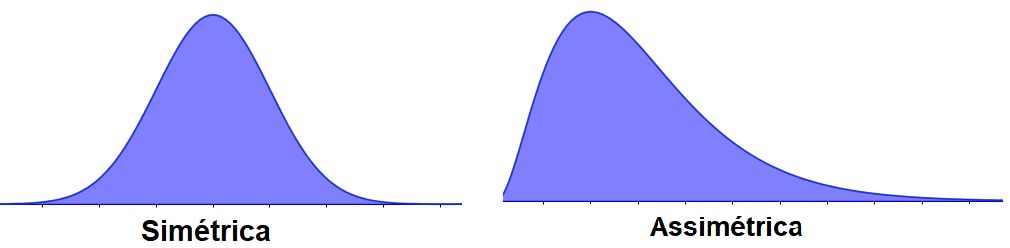
\includegraphics[scale=.5]{figuras/simetria}
\end{figure}
\noindent cujo temos por classificação, para uma distribuição unimodal:
	\begin{enumerate}
	    \item[(i)] \textbf{Simétrica}: se $Mo = Md = \overline{\mathnormal{x}}$;
		\item[(ii)] \textbf{Assimétrica positiva}: se $Mo < Md < \overline{\mathnormal{x}}$;
		\item[(iii)] \textbf{Assimétrica negativa}: se $\overline{\mathnormal{x}} < Md < Mo$.
	\end{enumerate}
\inic Para mensurar a simetria de uma distribuição este temos dois coeficientes, denominados 1º e 2º coeficientes de Pearson definidos por:

    \begin{equation}
	    AS = \frac{\overline{x} - Mo}{\sigma},
    \end{equation}
	ou
	\begin{equation}
	    AS = \frac{Q_1 + Q_3 - 2Md}{Q_3-Q_1}.
	\end{equation}
	Onde temos que:
	\begin{itemize}
	    \item $AS = 0$ a distribuição é simétrica;
	    \item $AS > 0$ a distribuição é simétrica positiva;
	    \item $AS < 0$ a distribuição é simétrica negativa.
	\end{itemize}
\subsection{Curtose}
\inic Denomina-se \textit{curtose} o grau de achatamento da distribuição, que pode ser classificada como:
\begin{enumerate}
	\item[(i)] \textbf{Platicúrtica}: Uma distribuição achatada, isto é, possui um ``bico" menos acentuado.
	\item[(ii)] \textbf{Leptocúrtica}: Uma distribuição delgada, ou seja, possui um ``bico" mais acentuado;
    \item[(iii)] \textbf{Mesocúrtica}: Uma distribuição nem chata nem delgada;
\end{enumerate}
\begin{figure}[H]
	\centering
	\caption{Classificação quanto à curtose}
	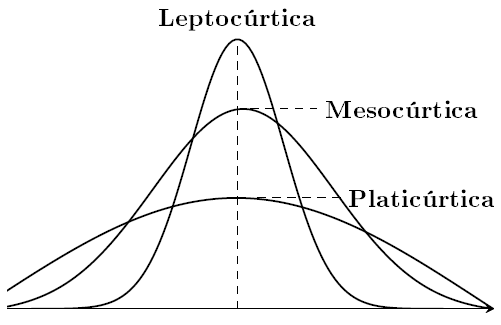
\includegraphics[scale=.9]{figuras/curtose}
\end{figure}
\subsubsection{Grau de curtose}
\inic Para medir o grau de curtose utiliza-se o coeficiente:
	\begin{equation}
	K = \frac{Q_1-Q_3}{2(P_{90} - P_{10})},    
	\end{equation}
	considerando a classificação:
	\begin{enumerate}
		\item[(i)] Se $K =0,263$, diz-se distribuição mesocúrtica; 
		\item[(ii)] Se $K>0,263$, diz-se distribuição platicúrtica;
		\item[(iii)] Se $K<0,263$, diz-se distribuição leptocúrtica.
	\end{enumerate}
\noindent \exemplo

\begin{enumerate}
	\item[(i)] Num teste aplicado a 20 alunos, obteve-se a seguinte distribuição de pontos:
	\begin{equation*}
	    \begin{tabular}{|c|c|c|c|c|c|c|c}
		    35 $\vdash$ 45 & 45 $\vdash$ 55 & 55 $\vdash$ 65 & 65 $\vdash$ 75 & 75 $\vdash$ 85 & $85 \vdash \hspace{-0.2 cm }\dashv 95$ \\ 
		    \hline
		    1&3&8&3&3&2\\
	    \end{tabular}
	\end{equation*}
	\begin{enumerate}
		\item[(a)] Calcular o desvio médio; 
		\item[(b)] Determinar a variância populacional;
		\item[(c)] Determinar o desvio padrão;
		\item[(d)] Classifique a distribuição quanto a assimetria e curtose.
	\end{enumerate}
\end{enumerate}
	
% \section{Teorema da Probabilidade Total}
% \section{O Teorema de Bayes}
% \section{Variáveis aleatórias}
% \subsection{Distribuição de probabilidade}
% \subsection{Esperança Matemática}
% \subsection{Variância}
% \chapter{Amostragem}

% \chapter{Teoria da Estimação}

% \chapter{Teoria da Decisão}

% \chapter{Modelos de Regressão}

% \chapter{Aplicações}

% \section{Aplicações à Administração}
% \section{Aplicações à Física}
% \section{Aplicações à Análise de Reflorestamento}
% \section{Aplicação à Propagação de Doenças}
\setcounter{chapter}{1} \chapter{Probabilidade}
\inic Neste capítulo, abordaremos os conceitos fundamentais da teoria das probabilidades, que constituem a base para o entendimento da inferência estatística. Em particular, na parte matemática, haverá momentos de maior rigor teórico. De modo geral, a probabilidade é amplamente aplicável em diversas áreas do conhecimento, tanto em pesquisas quantitativas quanto qualitativas. O objetivo deste capítulo é apresentar a probabilidade em nível de graduação, com ênfase em situações-problema relacionadas às áreas mencionadas no capítulo anterior.


\section{Histórico}
\inic A primeira manifestação foi dada por meio de jogos de dados, mas não é um dado qualquer era o conhecido como astrágalo, pequeno osso do tarso, situado entre a tíbia e o calcâneo. Este era usado como uma espécie de ``dado".

    \begin{figure}[h]
    \caption{Ástragalo}
		\centering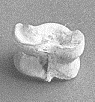
\includegraphics[scale=1]{figuras/astralagos}
	\end{figure}
	
\inic Usava-se o astrágalo para: previsão do futuro, divisão de heranças e disputas esportivas. As pesquisa na área de probabilidade iniciaram com Edmond Halley (1656 - 1665) e Girolamo Cardano (1570), quando estes estavam preocupados em fazer estimativas de taxas de seguro de vida. Depois disso, muito da teoria rigorosa foi desenvolvida pela família Bernoulli, mais especificamente com Daniel Bernoulli.

\section{Experimentos Aleatório}
\begin{defin}[Experimento aleatórios]
São aqueles que ao serem repetidos nas mesmas condições não produzem os mesmos resultados.
\end{defin}
\exemplo 
\begin{enumerate}
		\item[(i)] Retiradas de peças em um lote de peças numa fábrica, verificar quais são defeituosas;
		\item[(ii)] Escolher uma pessoa em um estádio de futebol para participar da partida;
		\item[(iii)] Verificar quantas toneladas de lixo foram depositados em um determinado local;
		\item [(iv)] Lançar um dado e verificar qual a face que se encontra voltada para cima;
		\item [(v)] Verificar se em um determinado dia choverá ou não.
	\end{enumerate}
Não são experimentos aleatórios
	\begin{enumerate}
		\item[(i)] Lançar uma pedra para o cima e verificar o que acontece;
		\item[(ii)] Dar partida num carro e verificar a distância percorrida após 10 segundos.
	\end{enumerate}
\inic Estaremos interessados em experimentos aleatórios, onde predomina a incerteza. 
\section{Espaço Amostral}
\begin{defin}[Espaço Amostral]
Denominamos espaço amostral associado a um experimento $\varepsilon$ o conjunto $\mathnormal{S}$ ou $\mathnormal{\Omega}$ de seus possíveis resultados.
\end{defin}
Isto é, listamos todos os possíveis resultados de um experimento aleatório temos o espaço amostral.

\exemplo
\begin{enumerate}
		\item[(i)] Lançamento de um dado possui espaço amostral $\mathnormal{\Omega} = \{1,2,3,4,5,6\}$;
		\item[(ii)]  Em uma moeda, represente $\mathnormal{K}$ o número de coroas e $\mathnormal{C}$ o número de cara. Verifica-se a face que caiu para cima, o espaço amostral é $\mathnormal{\Omega} = \{\mathnormal{C},\mathnormal{K}\}$;
		\item[(iii)] Sejam as condições do item (ii), suponha duas moedas, o espaço amostral é
		$$\mathnormal{\Omega} = \{\mathnormal{CC,CK,KC,KK}\}$$
		\item[(iv)] Três peças são retiradas de uma linha de produção. Cada peça é classificada como boa ($\mathnormal{B}$) ou defeituosa ($\mathnormal{D}$), o espaço amostral associado a esse experimento é dado por 
		$$\mathnormal{S} = \{\mathnormal{BBB, BBD, BDB,\dots, DDB, DDD}\}$$
		\item[(v)] Uma moeda é lançada até aparecer a primeira vez cara, o espaço amostral é
			$$\mathnormal{\Omega} = \{\mathnormal{C, KC, KKC, KKKC},\dots\}.$$
		\item [(vi)] Quantidade de pessoas que entram em uma determinada loja.
		\item [(vii)] Número de animais que existem em uma determinada região;
	\end{enumerate}
\inic Note que o espaço amostral dos itens (v) e (vi) são espaços de cardinalidade ($|\Omega|$) infinita, porém contável, pois não possui uma quantidade máxima de possíveis lançamentos e é possível enumerar estes elementos. Um espaço amostral que será muito útil é o do lançamento de dois dados, que é descrito por

\begin{equation}
\label{EAU}
	\mathnormal{\Omega}=\left[
	\begin{array}{cccccc}
	(1,1) & (1,2) & (1,3)& (1,4)&(1,5)&(1,6)\\
	(2,1) & (2,2) & (2,3)& (2,4)&(2,5)&(2,6)\\
	(3,1) & (3,2) & (3,3)& (3,4)&(3,5)&(3,6)\\
	(4,1) & (4,2) & (4,3)& (4,4)&(4,5)&(4,6)\\
	(5,1) & (5,2) & (5,3)& (5,4)&(5,5)&(5,6)\\
	(6,1) & (6,2) & (6,3)& (6,4)&(6,5)&(6,6)\\
	\end{array}
	\right]
\end{equation}
\begin{defin}[Evento]
 Chamamos de evento a todo resultado ou subconjunto de resultados de um experimento.
\end{defin}

\exemplo
\begin{enumerate}
	\item[(i)] No experimento de retirada de peças de um lote, seja o evento $\mathnormal{E}$: Retirar duas peças boas, o conjunto $\mathnormal{E}$ é dado por $\mathnormal{E}=\{\mathnormal{BBD}, \mathnormal{BDB}, \mathnormal{DBB}\}$;
	\item[(ii)] Considere o experimento lançar a moeda até dar cara, e defina os evento $\mathnormal{E}_1$: Dar cara no lançamento múltiplo de 2. Temos os conjuntos $\mathnormal{E}_1 = \{\mathnormal{KC,KKKC, KKKKKC,} \dots \}$;
	\item[(iii)] Escolhe-se um animal de um determinada região dada, temos o evento: ``o animal é uma felino".
	\item [(iv)] Em um conjunto de pessoas, escolhe-se uma ao acaso, e temos o evento: ``A pessoa é mulher"
\end{enumerate}
\inic Nosso objetivo é modelar os eventos e comparar com o espaço amostral. Calcular probabilidades é medir um fato aleatório e descrevermos qual destes é mais provável de ocorrer tal atitude ajuda a na tomada de decisões.

\subsection{Operações com Eventos}
\begin{enumerate}
	\item [(i)] A reunião de dois eventos $\mathnormal{A}$ e $\mathnormal{B}$, denotada por $\mathnormal{A \cup B}$ é o evento que ocorre se pelo menos um deles ocorre; 
	
	\begin{figure}[H]
    \caption{União de dois eventos}
		\centering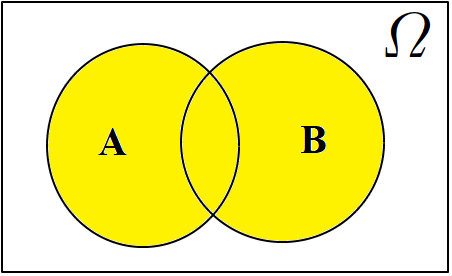
\includegraphics[scale=1]{figuras/uniao}
	\end{figure}
	
	\item [(ii)] A interseção de dois eventos $\mathnormal{A}$ e $\mathnormal{B}$, denotada por $\mathnormal{A} \cap \mathnormal{B}$, é o evento que ocorre quando ambos ocorrem;
	
	\begin{figure}[H]
    \caption{União de dois eventos}
		\centering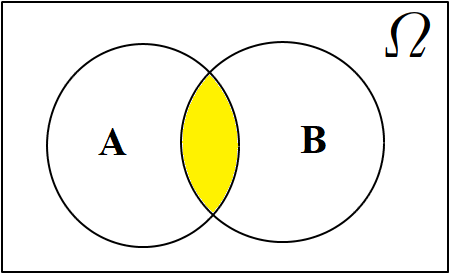
\includegraphics[scale=1]{figuras/inter}
	\end{figure}
	
	\item [(iii)] O complementar de um evento $\mathnormal{A}$, denotado por $\mathnormal{A}^c$ ou $\mathnormal{\overline{A}}$ é o evento que ocorre quando $\mathnormal{A}$ não ocorre.
	\begin{figure}[H]
            \caption{Evento Complementar}
		\centering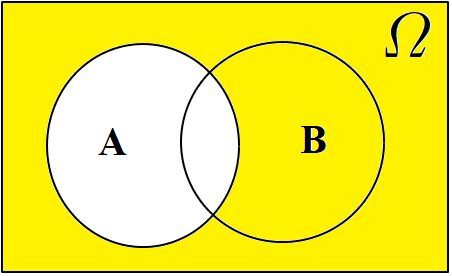
\includegraphics[scale=1]{figuras/comp.png}
	\end{figure}
\end{enumerate}
\inic Note que para (iii) a interseção não está em $A^c$ apesar de estar em $B$. Outra observação importante é que se $A\cap B = \phi$ então chamamos $A$ e $B$ de mutuamente exclusivos, isto é, eventos que não podem ocorrer juntos. Agora apresentaremos o Lema \ref{lema1} que pode ser muito útil quando se fala em manipulações com conjuntos. 

\begin{lema}
\label{lema1} Sejam $\mathnormal{A,B}$ e $\mathnormal{C}$ eventos de um espaço amostral $\mathnormal{\Omega}$, são válidas as relações
    \begin{enumerate}
		\item[(i)] $(\mathnormal{A\cup B})\cap \mathnormal{C} = (\mathnormal{A\cap C})\cup (\mathnormal{B \cap C})$;
		\item[(ii)] $\mathnormal{(A\cap B)\cup C = (A\cup C)\cap (B \cup C)}$;
		\item[(iii)] $\mathnormal{(A \cup B)^c = A^c \cap B^c}$;
		\item[(iv)] $\mathnormal{(A \cap B)^c = A^c \cup B^c}$.
	\end{enumerate}
\end{lema}
\inic A demonstração do Lema \ref{lema1} é facilmente encontrada em \cite{magalhaes2006probabilidade}, e também pode ser notada na forma dos diagramas de Veen. Faremos agora uma breve análise ``filosófica" a respeito do conceito de probabilidade esta que tem diversas abordagens. 

\section{Probabilidade Subjetiva}
\inic É a probabilidade que é baseada na crença do observador.
	\begin{enumerate}
		\item[(i)] Qual a probabilidade de chover hoje às 17:00?
		\item[(ii)] Qual a probabilidade de um clube ganhar todos os jogos da temporada?
		\item[(iii)] Qual a probabilidade de uma mulher grávida parir em um ambulância verde, no estado de Goiás às 19:00 de uma quinta feira;
		\item[(iv)] Qual a probabilidade do professor Andrey encontrar algum aluno para tomar café preto em baixo da torre de Pisa.
	\end{enumerate}
    
   Quando se trata de probabilidade subjetiva, cada observador possui uma crença distinta ou, em casos raros, semelhante; isto é, a opinião do pesquisador é levada em consideração. Embora, em alguns casos, essa abordagem possa ser eficiente, ela apresenta um caráter científico bastante limitado.
 
\section{Probabilidade Axiomática - Komogorov}

Probabilidade de um evento $\mathnormal{A}$, denotada por $\mathbb{P}(\mathnormal{A})$,  é uma função definida em uma classe de eventos $\mathcal{F}$ de $\mathnormal{\Omega}$ que satisfaz as seguintes condições:	
	\begin{enumerate}
		\item[(i)] $\mathbb{P}(\mathnormal{A}) \geq 0$;
		\item[(ii)] Se $(\mathnormal{A_n})_{\mathnormal{n} \geq 1}$ é uma sequência de eventos de $\mathcal{F}$, que são mutuamente exclusivo, então:
		\begin{equation*}	        \mathbb{P}\left(\bigcup_{\mathnormal{n}\geq 1}\mathnormal{A_n}\right) =  \displaystyle \sum_{\mathnormal{n}\geq 1} \mathbb{P}(\mathnormal{A_n}), 
			\end{equation*}
			em particular $\mathbb{P}(\mathnormal{A}_1 \cup \mathnormal{A}_2) = \mathbb{P}(\mathnormal{A}_1) + \mathbb{P}(\mathnormal{A}_2)$
			\item[(iii)] $\mathbb{P}(\mathnormal{\Omega}) = 1$.
		\end{enumerate}
\inic Com base nesses axiomas, podemos admitir que $0 \leq \mathbb{P}(A) \leq 1$ para qualquer evento $A$. Em outras palavras, a probabilidade de um evento será, no máximo, 1 (evento certo) e, no mínimo, 0 (evento impossível). A abordagem axiomática da probabilidade tem como principal objetivo estabelecer bases rígidas para o estudo de fenômenos aleatórios, ou seja, definir regras que devem ser respeitadas para que a teoria mantenha sua coerência dentro da lógica científica.


\section{Probabilidade Frequentista}

Seja um evento $\mathnormal{A}$ e $\mathnormal{n(A)}$ o número de vezes em que o evento $\mathnormal{A}$ ocorreu nas $|\Omega|=\mathnormal{N}$ repetições do experimento. Denominamos probabilidade de $\mathnormal{A}$, denotada por $\mathbb{P}(\mathnormal{A})$, à razão: 
	\begin{equation*}
			\mathbb{P}(\mathnormal{A}) = \frac{\mathnormal{n(A)}}{\mathnormal{N}}.
		\end{equation*}
        
	Uma pergunta que pode surgir é: por que não usar sempre a probabilidade baseada em frequências, já que ela é a abordagem mais experimental possível? A resposta é simples: nem sempre isso é viável. Para que um pesquisador utilize a probabilidade frequentista, é necessário que o experimento aleatório seja realizado sempre nas mesmas condições, o que muitas vezes é impraticável — para não dizer impossível. Um exemplo típico é o cálculo da probabilidade de um ser humano sobreviver a uma cirurgia. Não é possível realizar esse experimento sob condições idênticas, considerando diversos fatores que variam de uma cirurgia para outra, como a idade do paciente.

	
	
\exemplo
\begin{enumerate}
	  \item [(i)] O espaço amostral do lançamento de uma moeda equilibrada é $\mathnormal{\Omega} = \{C,K\}$, a probabilidade de dar cara ou coroa é $\mathbb{P}(C) = \mathbb{P}(K)= \dfrac{1}{2}$;
	  \item [(ii)] O espaço amostral do lançamento de um dado equilibrado é $\mathnormal{\Omega} = \{1,2,3,4,5,6\}$ a probabilidade de cair a face $i$ voltada para cima é $\mathbb{P}(i) = \dfrac{1}{6}$.
\end{enumerate}

\exemplo 

\begin{enumerate}
		\item[(i)]No lançamento de dois dados equilibrados, determine
		\begin{enumerate}
			\item[(a)] A probabilidade de dar par em ambos os dados;\\
			Use o espaço \ref{EAU}, onde já sabemos que $|\Omega| = 36$ e agora temos que selecionar os subconjuntos em que no primeiro lançamento e no segundo temos apenas números pares, isto é, $n(Os\,\,dois\,\, pares) = 9$, assim $\mathbb{P}(Os\,\,dois\,\, pares)=\dfrac{9}{36}=\dfrac{1}{4}$
			\item [(b)] A probabilidade de dar dois impares;\\
			\inic Tome o mesmo raciocínio do item (a), logo $\mathbb{P}(Os\,\,dois\,\, impares)=\dfrac{9}{36}=\dfrac{1}{4}$
			\item [(c)] A probabilidade da soma ser 8;\\
			Note que todas as ``diagonais secundárias" a soma igual um valor de 2 (soma mínima) à 12 (soma máxima), basta encontramos $A = \{(2,6), (3,5), (4,4), (5,3), (6,2)\}$, logo a $\mathbb{P}(A) = \dfrac{n(A)}{N}=\dfrac{4}{36} = \dfrac{1}{9}$.
		\end{enumerate}
		\item[(ii)] No lançamento de duas moedas, determine
		\begin{enumerate}
			\item [(a)] A probabilidade de dar cara em uma e coroa na outra;\\
			Note que o $\Omega = \{(K,K), (C,K), (K,C), (C,C)\}$, logo aqui $|\Omega| = 4$ e queremos os casos $A = \{(C,K), (K,C)\}$ logo $|A| = 2$ assim $\mathbb{P}(A) = \dfrac{1}{2}$
			\item [(b)] É feito duas vezes o lançamento das duas moedas, qual a probabilidade de dar cara em todas?
		\end{enumerate}
	 \item[(iii)] Um número inteiro é escolhido aleatoriamente dentre os números $1,2,3,\dots,50$, qual a probabilidade de
	\begin{enumerate}
		\item [(a)] O número ser divisível por 5;\\
		Basta verificar que $A_1 = \{5,10,15,20,\dots,50\}$ são divisíveis por $5$logo temos $|A_1| = 10$, assim $\mathbb{P}(A_1) = \dfrac{10}{50} = \dfrac{1}{5}$
		\item [(b)] Terminar em 3;\\
		Basta fazer a contagem do conjuntos $A_2 = \{3,13,23,33,43\}$, logo $\mathbb{P}(A_2) = \dfrac{10}{50} = \dfrac{5}{50} = \dfrac{1}{10}$
		\item [(c)] Terminar em impar e não começar em par\\
		O conjunto descrito acima é
		$$A_3 = \{\text{os números impares que tem o primeiro digito impar}\}$$ 
		logo $|A_3|= 15$, assim $\mathbb{P}(A_3) = \dfrac{15}{50}= \dfrac{3}{10}$.
 	\end{enumerate}
 	\end{enumerate}
\section{Alguns resultados importantes}

Alguns resultados são fundamentais para a resolução de problemas probabilísticos. Um deles é o cálculo da probabilidade do evento complementar, apresentado na Proposição \ref{complementar}.
 \begin{prop}
Sejam $A$ e $B$ eventos de um espaço de probabilidade $(\Omega,\mathcal{F},\mathbb{P})$. Então valem as seguintes propriedades:

\begin{enumerate}
    \item[(i)] (Complemento) Se $A^c$ é o complementar de $A$, então
    \begin{equation}
        \mathbb{P}(A) = 1 - \mathbb{P}(A^c).
    \end{equation}

    \item[(ii)] (Monotonicidade) Se $A \subset B$, então
    \begin{equation}
        \mathbb{P}(A) = \mathbb{P}(B) - \mathbb{P}(B \setminus A),
    \end{equation}
    e, em particular,
    \begin{equation}
        \mathbb{P}(A) \leq \mathbb{P}(B).
    \end{equation}

    \item[(iii)] (Inclusão-Exclusão) Para quaisquer eventos $A$ e $B$,
    \begin{equation}
        \mathbb{P}(A \cup B) = \mathbb{P}(A) + \mathbb{P}(B) - \mathbb{P}(A \cap B).
    \end{equation}
\end{enumerate}
\end{prop}

\begin{proof}
Vamos demonstrar cada item separadamente.

\begin{enumerate}
    \item[(i)] Como $A \cup A^c = \Omega$ e $A \cap A^c = \emptyset$, aplicando os axiomas de Kolmogorov, temos
    \begin{align*}
        \mathbb{P}(A \cup A^c) &= \mathbb{P}(\Omega) = 1, \\
        \mathbb{P}(A) + \mathbb{P}(A^c) &= 1,
    \end{align*}
    donde segue
    \begin{equation*}
        \mathbb{P}(A) = 1 - \mathbb{P}(A^c).
    \end{equation*}

    \item[(ii)] Se $A \subset B$, então $B = A \cup (B \setminus A)$, com união disjunta. Logo,
    \begin{align*}
        \mathbb{P}(B) &= \mathbb{P}(A) + \mathbb{P}(B \setminus A), \\
        \mathbb{P}(A) &= \mathbb{P}(B) - \mathbb{P}(B \setminus A).
    \end{align*}
    Como $\mathbb{P}(B \setminus A) \geq 0$, segue que
    \begin{equation*}
        \mathbb{P}(A) \leq \mathbb{P}(B).
    \end{equation*}

    \item[(iii)] Note que
    \begin{equation*}
        A \cup B = (A \setminus B) \cup (B \setminus A) \cup (A \cap B),
    \end{equation*}
    união disjunta. Logo,
    \begin{equation}
        \mathbb{P}(A \cup B) = \mathbb{P}(A \setminus B) + \mathbb{P}(B \setminus A) + \mathbb{P}(A \cap B).
    \end{equation}
    
    Além disso,
    \begin{align*}
        \mathbb{P}(A) &= \mathbb{P}(A \setminus B) + \mathbb{P}(A \cap B), \\
        \mathbb{P}(B) &= \mathbb{P}(B \setminus A) + \mathbb{P}(A \cap B).
    \end{align*}
    Somando as duas expressões,
    \begin{align*}
        \mathbb{P}(A) + \mathbb{P}(B)
        &= \mathbb{P}(A \setminus B) + \mathbb{P}(B \setminus A) + 2\mathbb{P}(A \cap B).
    \end{align*}
    Substituindo na expressão de $\mathbb{P}(A \cup B)$, obtemos
    \begin{equation*}
        \mathbb{P}(A \cup B) = \mathbb{P}(A) + \mathbb{P}(B) - \mathbb{P}(A \cap B).
    \end{equation*}

\end{enumerate}
\end{proof}

\section{Probabilidade Condicional}
    
 Em linhas gerais, estudar a probabilidade condicional significa analisar eventos que são dependentes uns dos outros. Quando enfrentamos um evento muito complexo para modelar, uma alternativa para solucionar o problema é condicioná-lo a eventos mais simples, facilitando assim a análise. Outro ponto importante sobre condicionar eventos é que, em geral, buscamos reduzir o esforço de contagem e/ou modelagem de parte do espaço amostral.


\exemplo
\begin{enumerate}
    \item [(i)] Considere o problemas clássico do lançamento de dois dados, onde já descrevemos o espaço amostral por,
\begin{equation}
    \label{EAU1}
	\mathnormal{\Omega}=\left[
	\begin{array}{cccccc}
	(1,1) & (1,2) & (1,3)& (1,4)&(1,5)&(1,6)\\
	(2,1) & (2,2) & (2,3)& (2,4)&(2,5)&(2,6)\\
	(3,1) & (3,2) & (3,3)& (3,4)&(3,5)&(3,6)\\
	(4,1) & (4,2) & (4,3)& (4,4)&(4,5)&(4,6)\\
	(5,1) & (5,2) & (5,3)& (5,4)&(5,5)&(5,6)\\
	(6,1) & (6,2) & (6,3)& (6,4)&(6,5)&(6,6)\\
	\end{array}
	\right],
\end{equation}
ou seja, o problema busca estudar o comportamento dos pares ordenados  colocados na Matriz (\ref{EAU1}). Note que sem nenhuma informação previa temos que a probabilidade de cada ponto do espaço amostral é $\dfrac{1}{36}$. Mas agora, vamos supor que antes do lançamento do segundo dado tem-se a informação que o número de face para cima é maior que igual à 3, daí com esta informação exclui-se a possibilidade dos pares da primeira e segunda linha, isto é, teremos $|\Omega| = 4 \times 5 = 20$, logo as probabilidade serão
\begin{equation}
    \mathbb{P}(A) = \begin{cases}
    1/20, \text{se o par pertence a linhas  $\geq$ 3}\\
    0, \text{caso contrário}
    \end{cases}.
\end{equation}
\inic Então, note que uma informação a respeito do processo aleatório mudou o comportamento probabilístico do pontos do espaço, esse tipo de modificação que estudaremos nesta seção.
\end{enumerate}	
\begin{defin}{(Probabilidade condicional)}
    Seja $A$ e $B$ dois eventos de $\Omega$ com $\mathbb{P}(A) > 0$ definimos $\mathbb{P}(B|A)$, a probabilidade do evento $B$ dado $A$, por
    \begin{equation}
        \mathbb{P}(B|A) = \dfrac{\mathbb{P}(B\cap A)}{\mathbb{P}(A)},
    \end{equation}
\end{defin}
buscando o contexto do exemplo anterior o evento $A:$ a primeira face é maior que 3 e $B:$ cada ponto do espaço amostral.

\exemplo
\begin{enumerate}
    \item [(i)] Suponha que uma estação de rádio tenha amostrado 100 pessoas, 20 das quais tinham crianças. Eles observaram que 30 dessas pessoas usavam cinto de segurança, e que 15 daquelas pessoas tinham crianças. Os resultados são mostrados na Tabela \ref{cinto}
    
    \begin{table}[H]
        \centering
        \caption{Uso de cinto}
        \label{cinto}
        \begin{tabular}{|c|c|c|c|}
	    \hline
	    Paternidade & Usam cinto & Não usam cinto & Total\\
	    \hline
	        Com crianças & 15 & 5 & 20\\
	        Sem Crianças & 15 & 65 & 80\\
	        Total & 30 & 70 & 100\\
	        \hline
        \end{tabular}
\end{table}
    Qual a probabilidade de uma pessoa tendo criança usar cinto de seguranças? Qual a probabilidade de uma pessoa tendo criança não usar cinto? Usaremos a definição de probabilidade condicional para determinar estas probabilidades, logo definimos os eventos:
    \begin{equation}
        \begin{cases}
            A: \text{Usar cinto de segurança}\\
            B: \text{Ter criança}
        \end{cases}
    \end{equation}
    Então temos que $\mathbb{P}(A \cap B) = \dfrac{15}{100}$ e $\mathbb{P}(B) = \dfrac{20}{100}$ 
\begin{align*}
    \mathbb{P}(A|B) &= \dfrac{15/100}{20/100} \\ 
    &=\dfrac{15}{20} = 3/4.
\end{align*}
Uma estratégia para calcularmos a probabilidade da segunda pergunta é usarmos o evento complementar, note que como a condição é em cima do mesmo evento, temos a seguinte relação
    \begin{align*}
        \mathbb{P}(A^c|B) &= 1 - \mathbb{P}(A|B)\\
        &= 1 - 3/4 = 1/4.
    \end{align*}
\end{enumerate}	
Formalizaremos agora algumas propriedades de probabilidade condicional por meio do Lema

\begin{prop}
     Seja $\mathnormal{A}$ um evento tal que $\mathbb{P}(\mathnormal{A})>0$. A probabilidade condicional satisfaz:
	\begin{enumerate}
		\item[(i)]$\mathbb{P}(\mathnormal{B|A}) \geq 0$;
		\item[(ii)] Se $(\mathnormal{B_n})_{\mathnormal{n} \geq 1}$ é uma sequência de eventos de $\mathcal{F}$, que são mutuamente exclusivo, então:
		\begin{equation*}
		\mathbb{P}(\bigcup_{\mathnormal{n}=1}^{\mathnormal{n}}\mathnormal{B_k}|\mathnormal{A}) =  \displaystyle \sum_{\mathnormal{i}=1}^{\mathnormal{n}} \mathbb{P}(\mathnormal{B_k|A}); 
		\end{equation*}
		\item[(iii)] $\mathbb{P}(A^c|B) = 1 - \mathbb{P}(A|B)$
		\item[(iv)] $\mathbb{P}(\mathnormal{\Omega}|\mathnormal{\Omega}) = 1$.
	\end{enumerate}
\end{prop}
\section{Teorema da Probabilidade Total}
Em alguns casos condicionar o evento em apenas um evento mais simples, não é viável, algumas vezes nem mesmo é possível, para os casos em que necessitamos fazer o condicionamento em diversos eventos, mais precisamente uma sequência de eventos usamos o teorema da probabilidade total.
\begin{teo}{(Probabilidade Total)}
\label{probtotal}
Seja $\mathnormal{B}_1, \mathnormal{B}_2, \mathnormal{B}_3, \dots, \mathnormal{B_n}$ uma partição de  $\mathnormal{\Omega}$, isto é, são eventos mutuamente excludentes e a sua reunião é $\mathnormal{\Omega}$. Seja $\mathnormal{A}$ um evento e $\mathbb{P}(\mathnormal{A})$ uma probabilidade definida nos eventos de $\mathnormal{\Omega}$, temos:
	\begin{equation*}
		\mathbb{P}(\mathnormal{A}) = \displaystyle \sum_{\mathnormal{i}=1}^{\mathnormal{n}}\mathbb{P}(\mathnormal{A|B_i})\mathbb{P}(\mathnormal{B_i})
	\end{equation*}
\end{teo}
	Em suma, o Teorema \ref{probtotal} é extremamente útil quando o espaço amostral está $n$ particionado note o exemplo

\exemplo
	 \begin{enumerate}
	     \item [(i)] Dadas as urnas $\mathnormal{U}_1, \mathnormal{U}_2$ e $\mathnormal{U}_3$ com as seguintes composições: a $\mathnormal{U}_1$ tem 3 bolas brancas e 5 bolas vermelhas, a $\mathnormal{U}_2$ tem 4 brancas e 2 vermelhas e a $\mathnormal{U}_3$ tem tem 1 branca e 3 vermelhas. Escolhe-se uma das três urnas sendo: $\mathbb{P}(\mathnormal{U}_1) = 2/6$, $\mathbb{P}(\mathnormal{U}_2) = 3/6$ e $\mathbb{P}(\mathnormal{U}_3) = 1/6$, retira-se uma bola, determine a probabilidade desta ser branca. 
	     
	     \inic Note que o espaço de bolas brancas está dividido em 3 urnas ($U_1, U_2, U_3$) logo para este caso temos $n=3$. a probabilidade de cada urna é dada no problema então, seja $A$: retirar uma bola branca. Logo
	         \begin{align*}
	              \mathbb{P}(\mathnormal{A}) &= \displaystyle \sum_{\mathnormal{i}=1}^{\mathnormal{3}}\mathbb{P}(\mathnormal{A|B_i})\mathbb{P}(\mathnormal{B_i})\\
	              &= \displaystyle \mathbb{P}(\mathnormal{A|U_1})\mathbb{P}(\mathnormal{U_1}) + \mathbb{P}(\mathnormal{A|U_2})\mathbb{P}(\mathnormal{U_2}) + \mathbb{P}(\mathnormal{A|U_3})\mathbb{P}(\mathnormal{U_3})\\
	              &= \dfrac{3}{8}.\dfrac{2}{6} + \dfrac{4}{6}.\dfrac{3}{6} + \dfrac{1}{4}.\dfrac{1}{6}
	         \end{align*}
	     
	     \item[(ii)] Um piloto tem 50\% de probabilidade de vencer uma corrida sob chuva. Caso não chova tem probabilidade de vitória de 25\%. A meteorologia estima 30\% a probabilidade de chuva durante a corrida, qual a probabilidade do piloto ganhar a corrida?
	 \end{enumerate}
	
\begin{teo}{(De Bayes)}
Seja $\mathnormal{B}$ um evento e $\mathnormal{A}_1,\dots, \mathnormal{A_n}$ partições do espaço amostral $\mathnormal{\Omega}$, seja $\mathbb{P}$ uma probabilidade definida em $\mathnormal{\Omega}$, temos:
	\begin{equation*}
		\mathbb{P}(\mathnormal{A_i|B}) = \frac{\mathbb{P}(\mathnormal{B|A_i})\mathbb{P}(\mathnormal{A_i})}{\displaystyle \sum_{\mathnormal{i}=1}^{\mathnormal{n}}\mathbb{P}(\mathnormal{B|A_i})\mathbb{P}(\mathnormal{A_i})}
	\end{equation*} 
\end{teo}
\inic O principal objetivo do Teorema de Bayes é calcular a probabilidade de uma partição de $\Omega$ tendo conhecimento do evento $B$.

\chapter{Variáveis Aleatórias}
\section{Conceito}

 Este capítulo tem por objetivo construir uma das principais — senão a principal — partes da teoria das probabilidades: o conceito de variáveis aleatórias, um objeto matemático fundamental para resolver diversos problemas práticos nas áreas abordadas nestas notas. Em suma, estudar variáveis aleatórias é estudar funções que possuem propriedades muito especiais. vejamos alguns exemplos.\\

\exemplo
    \begin{enumerate}
        \item [(i)]
    Lance uma moeda 10 vezes e observe a sequência de caras que ocorreram, seria interessante determinarmos uma função que fizesse a contagem destas variáveis, pois bem esta tarefa é de uma variável aleatória. Uma sugestão é, construir a variável $X$ tal que:
    \begin{equation}
    \label{01}
        X(\omega):= \begin{cases}
            1,\,\,\text{se cara}\\
            0,\,\,\text{se coroa}, 
        \end{cases}
    \end{equation}
    atentemos as dois detalhes, estamos substituindo no nosso problema ``caras''  pelo número 1 pelo fato de estarmos interessados na contagem desta face da moeda. a variável X em questão não é a única forma de modelar o problema em questão, porém a a mais usual.
    \item[(ii)] Escolhe um ponto ao acaso no circulo unitário temos, $\Omega = \{(x,y): x^2 + y^2 \leq 1\}$ neste caso temos duas coordenadas a serem observadas, a coordenada $X$ e $Y$ que são sorteadas independente uma da outra.
    \item[(iii)] Uma área da engenharia possui bastante aleatoriedades é a parte de trânsito, podemos definir variáveis as quais façam contagem de carros que passam em uma determinada esquina que meça quantas pessoas atravessam uma faixa de trânsito ou pessoas que utilizam um determinado transporte público e etc. 
    \end{enumerate}

    \begin{defin}[Variáveis aleatórias]
        Uma variável aleatória é uma função $X: \Omega \rightarrow \mathbb{R}$ que associa cada elemento do espaço amostral a um único número real. 
    \end{defin}
    Tais variáveis são classificadas como \textit{Discretas}, \textit{Contínuas} ou \textit{Mistas}. Em suma, estamos tratando com funções que associam pontos do espaço amostral a um número. E porque acrescentar o nome ``aleatória"? Pelo fato para cada valor (ou área) destas variáveis atribui-se uma probabilidade de esta ocorrer.\\
    
    \exemplo
    
    Um jogo de dado com seis faces, pode ser entendido com uma variável aleatória, considere que todas as faces possuem a mesma probabilidade de ocorrência $1/6$ então $\Omega = \{f_1,f_2,f_3,f_4,f_5,f_6\}$ são todas as faces do dado. Podemos definir uma variável $Y$ tal que $Y(f_i):=i$ com $i = 1,\dots,6$, ou seja, cada face terá um número atribuído, conforme a figura 

        \begin{figure}[H]
            \caption{Diagrama variável $Y$}		\centering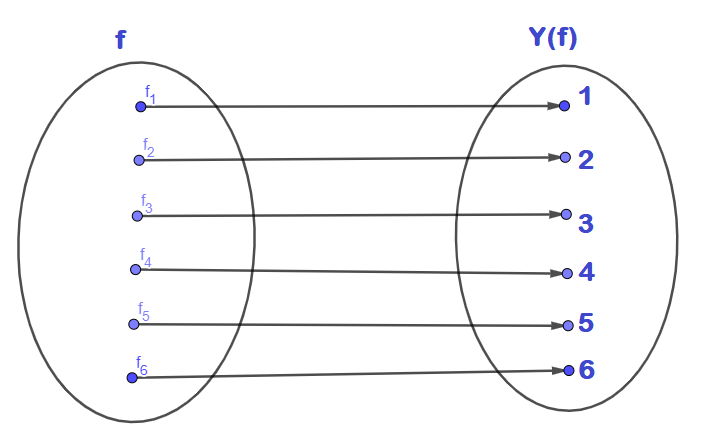
\includegraphics[scale=0.4]{figuras/va_dado.png}
	\end{figure}
 
    De forma semelhante, para a variável $X$ definida em \ref{01} temos 

        \begin{figure}[H]
            \caption{Diagrama variável $X$}
		\centering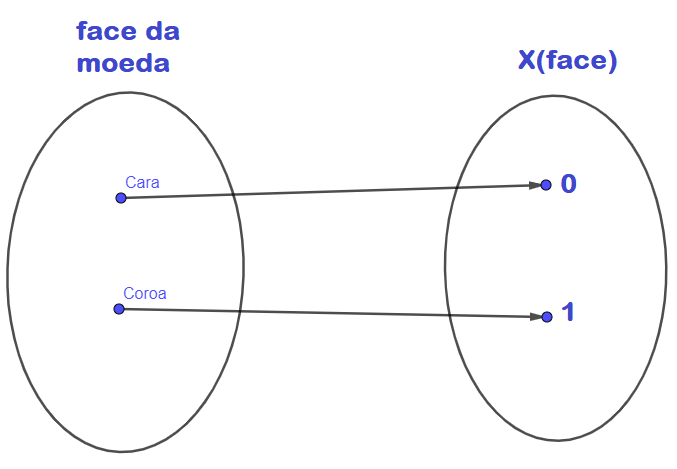
\includegraphics[scale=0.4]{figuras/va_moeda.png}
	\end{figure}

    Os dois modelos de exemplos citados são muito importantes, pois são demasiadamente citados em problemas probabilísticos e problemas de pesquisa.
    
\section{Distribuição de probabilidade}

Em linhas gerais, uma distribuição de probabilidade é uma tabela que apresenta todos os valores possíveis de uma variável aleatória juntamente com a probabilidade desses valores ocorrerem, em geral para começar a estudar bem um problema probabilístico precisamos ter bem definida a distribuição de probabilidade das variáveis em questão, por exemplo, as variáveis $X$ e $Y$ definidas anteriormente possuem as seguintes distribuições

\begin{table}[H]
        \centering
        \label{cinto}
        \begin{tabular}{c|c|c}
	    X & 0 & 1\\
	    \hline
	    $\mathbb{P}(X=x)$ & $1/2$ & $1/2$     
        \end{tabular}
    \end{table}
e 
\begin{table}[H]
    \centering
    \label{cinto}
    \begin{tabular}{c|c|c|c|c|c|c}
	Y & 1 & 2 & 3&4&5&6\\
	\hline
	$\mathbb{P}(Y=y)$ & $1/6$ & $1/6$ & $1/6$ & $1/6$ & $1/6$ & $1/6$    
    \end{tabular}
\end{table}
\inic Observe que a somas das probabilidades tem que ser sempre 1. Imagine que vamos unir esse dois jogos, então não estamos mais interessados na variáveis separada estamos por exemplo interessados em $X+Y$, como ficaria a distribuição? sendo a moeda independente do dado. 
Os possíveis valores para $Z=X+Y$ são $\{1,2,\dots,7\}$, pois podemos ter no mínimo o dado assumindo 1 e a moeda 0, bem como no máximo o dado assumindo 6 e a moeda 1, logo temos 
\begin{equation*}
    \begin{cases}
        \mathbb{P}(Z = 1) = \mathbb{P}(X=0)\mathbb{P}(Y=1) = \dfrac{1}{2}.\dfrac{1}{6} = \dfrac{1}{12}\\
        \mathbb{P}(Z = 2) = \mathbb{P}(X=0)\mathbb{P}(Y=2) + \mathbb{P}(X=1)\mathbb{P}(Y=1) = \dfrac{1}{2}.\dfrac{1}{6} + \dfrac{1}{2}.\dfrac{1}{6} = \dfrac{2}{12}\\
        \mathbb{P}(Z = 3) = \mathbb{P}(X=0)\mathbb{P}(Y=3) + \mathbb{P}(X=1)\mathbb{P}(Y=2) = \dfrac{1}{2}.\dfrac{1}{6} + \dfrac{1}{2}.\dfrac{1}{6} = \dfrac{2}{12}\\
        \vdots\\
        \mathbb{P}(Z = 6) = \mathbb{P}(X=0)\mathbb{P}(Y=6) + \mathbb{P}(X=1)\mathbb{P}(Y=5) = \dfrac{1}{2}.\dfrac{1}{6} + \dfrac{1}{2}.\dfrac{1}{6} = \dfrac{2}{12}\\
        \mathbb{P}(Z = 7) = \mathbb{P}(X=0)\mathbb{P}(Y=6) = \dfrac{1}{2}.\dfrac{1}{6} = \dfrac{1}{12}
    \end{cases}
\end{equation*}
Assim a distribuição será
\begin{table}[H]
    \centering
    \label{cinto}
    \begin{tabular}{c|c|c|c|c|c|c|c}
	Z & 1 & 2 & 3&4&5&6& 7\\
	\hline
	$\mathbb{P}(Z=z)$ & $1/12$ & $2/12$ & $2/12$ & $2/12$ & $2/12$ & $2/12$ & $1/12$    
    \end{tabular}
\end{table}
Assim, um jogo com a dinâmica da variável $Z$ os números que não são indicados apostar são $Z=1$ e $Z=7$, pois são os menos prováveis de acontecer. Podemos representar essa dinâmica via função escada.
        \begin{figure}[H]
            \caption{Diagrama variável $X$}
		\centering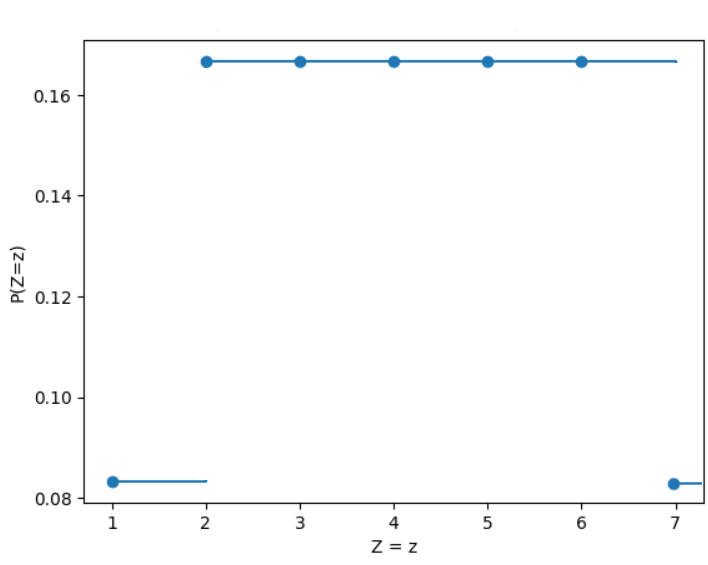
\includegraphics[scale=0.5]{figuras/va_Z.png}
	\end{figure}
    
Observe que esta estrutura de gráfico e tabelas para representar as distribuições de probabilidade não são uteis para variáveis contínuas, e para estas usaremos outra representação. 

\section{Função densidade de probabilidade}
	As funções densidade de probabilidade desempenham, no caso de variáveis aleatórias contínuas, um papel semelhante ao das funções de probabilidade no caso discreto. A principal diferença é que, para uma variável aleatória contínua, as probabilidades não são atribuídas diretamente a valores isolados, mas sim a \textbf{intervalos } do conjunto dos números reais.

Em outras palavras, se \(X\) é uma variável aleatória contínua, uma função \(f_X:\mathbb{R}\to\mathbb{R}\) será chamada de \textit{função densidade de probabilidade} de \(X\) se satisfizer as seguintes propriedades:

\begin{enumerate}
    \item[(i)] $ f_X(x)\geq 0,\qquad \forall x\in\mathbb{R},$\\
    \item[(ii)]$\int_{-\infty}^{+\infty}f_X(x),dx=1.$
\end{enumerate}

A probabilidade de \(X\) assumir um valor em determinado intervalo é obtida pela área sob a curva da função densidade nesse intervalo. Assim,

\begin{equation}
\mathbb P(a\leq X\leq b)=\int_a^b f_X(x),dx.
\end{equation}

Portanto, diferentemente do caso discreto, $f_X(x)$ não representa diretamente a probabilidade $\mathbb P(X=x)$. De fato, para uma variável aleatória contínua,

\begin{equation}
\mathbb P(X=x)=0,\qquad \forall x\in\mathbb{R}.
\end{equation}

Isso ocorre porque a probabilidade está associada à área de um intervalo, enquanto um único ponto possui comprimento nulo. Como consequência,

\begin{equation}
    \mathbb P(a<X<b)=\mathbb P(a\leq X<b)=\mathbb P(a<X\leq b)=\mathbb P(a\leq X\leq b).
\end{equation}

É importante observar ainda que a função densidade pode assumir valores maiores que \(1\). O que deve estar entre \(0\) e \(1\) é a probabilidade obtida pela integral da densidade sobre um conjunto, e não necessariamente o valor da própria função \(f_X(x)\).

\exemplo
\begin{enumerate}
    \item[(i)] A função $f(x)=-x^2$ no intervalo $[-1,1]$ não é uma função densidade, pois, para $x=1$, temos $f(1)=-1<0$, fato que por si só já elimina a possibilidade de $f$ ser uma função densidade. Além disso,
    \begin{equation}
    \int_{-1}^{1}-x^2,dx=-\left[\frac{x^3}{3}\right]_{-1}^{1}=-\left(\frac{1}{3}+\frac{1}{3}\right)=-\frac{2}{3}\neq 1.
\end{equation}
Portanto, a função viola as duas condições necessárias para ser uma função densidade de probabilidade.

\item[(ii)] Considere a função $f(x)=x+\frac{1}{2}$ no intervalo $[-1,1]$. Temos
\begin{equation}
\int_{-1}^{1}\left(x+\frac{1}{2}\right),dx
=\left[\frac{x^2}{2}+\frac{x}{2}\right]_{-1}^{1}=1.
\end{equation}
Portanto, a função satisfaz a condição de que a integral sobre todo o domínio seja igual a $1$. Entretanto, para $x=-1$, temos
\begin{equation}
f(-1)=-1+\frac{1}{2}=-\frac{1}{2}<0.
\end{equation}
Assim, $f$ não é uma função densidade, pois viola apenas a condição de não negatividade.

\item[(iii)] Considere agora a função $f(x)=x^2$ no intervalo $[-1,1]$. Como $x^2\geq0$ para todo $x\in[-1,1]$, a condição de não negatividade é satisfeita. Entretanto,
\begin{equation}
    \int_{-1}^{1}x^2\,dx
    =\left[\frac{x^3}{3}\right]_{-1}^{1}
    =\frac{2}{3}\neq1.
\end{equation}
Portanto, $f$ não é uma função densidade, pois, embora seja não negativa em todo o seu domínio, sua integral total é diferente de $1$.

\end{enumerate}

Ou seja, os exemplos (i), (ii) e (iii) mostram que nem toda função pode ser considerada uma função densidade de probabilidade. Portanto, antes de utilizarmos uma determinada função nesse contexto, devemos verificar se ela satisfaz as condições necessárias para ser classificada como uma função densidade de probabilidade.

\section{Esperança e Variância}

Até o momento, estudamos como descrever o comportamento de uma variável aleatória por meio de sua função de probabilidade, no caso discreto, ou de sua função densidade de probabilidade, no caso contínuo. Entretanto, muitas vezes estamos interessados em resumir algumas características importantes da distribuição utilizando apenas alguns valores numéricos.

Duas das medidas mais importantes para esse propósito são a \textbf{esperança} e a \textbf{variância}. De maneira intuitiva, a esperança procura indicar em torno de qual valor os possíveis resultados da variável aleatória estão distribuídos, enquanto a variância mede o quanto esses resultados tendem a se afastar desse valor.

\subsection{Esperança}

Seja $X$ uma variável aleatória. A \textbf{esperança matemática}, também chamada de \textbf{valor esperado} ou \textbf{média de $X$}, é uma medida que procura representar o valor médio da variável aleatória quando o experimento é repetido um grande número de vezes.

A esperança de $X$ será denotada por
\begin{equation}
\mathbb{E}[X]=\mu.
\end{equation}

É importante observar que $\mathbb{E}[X]$ não precisa ser um valor que a variável aleatória possa efetivamente assumir. Por exemplo, ao lançarmos um dado equilibrado, os possíveis resultados são $1,2,3,4,5$ e $6$, porém o valor esperado é $3,5$. Portanto, a esperança deve ser interpretada como uma medida de tendência central da distribuição, e não necessariamente como um possível resultado do experimento.

A maneira como calculamos $\mathbb{E}[X]$ depende do tipo da variável aleatória. Para variáveis discretas utilizamos uma soma ponderada pelas probabilidades, enquanto para variáveis contínuas utilizamos uma integral ponderada pela função densidade.

\subsubsection{Esperança de uma variável aleatória discreta}

Seja $X$ uma variável aleatória discreta que assume os valores $x_1,x_2,\ldots$ com função de probabilidade
\begin{equation}
\mathbb P(X=x_i)=p(x_i).
\end{equation}

A esperança de $X$ é definida por
\begin{equation}
    \mathbb{E}[X]=\sum_i x_i\mathbb P(X=x_i)
\end{equation}
desde que essa soma esteja bem definida.

Observe que cada possível valor $x_i$ é multiplicado pela probabilidade de sua ocorrência. Dessa forma, valores com maior probabilidade possuem maior influência sobre o valor da esperança.

Por exemplo, considere o lançamento de um dado equilibrado. Se $X$ representa o número observado na face superior, então
\begin{equation}
\mathbb P(X=x)=\frac{1}{6},\qquad x=1,2,\ldots,6.
\end{equation}
Consequentemente,
\begin{equation}
\mathbb{E}[X]=\sum_{x=1}^{6}x\mathbb P(X=x)=\frac{1}{6}(1+2+3+4+5+6)=\frac{21}{6}=3,5.
\end{equation}

Note que $3,5$ não é um possível resultado do lançamento de um dado. Esse valor representa o comportamento médio dos resultados quando imaginamos a repetição do experimento muitas vezes.

\subsubsection{Esperança de uma variável aleatória contínua}

No caso de uma variável aleatória contínua, não podemos calcular a esperança somando valores individuais, pois cada ponto possui probabilidade igual a zero. Nesse caso, utilizamos a função densidade de probabilidade.

Seja $X$ uma variável aleatória contínua com função densidade $f_X(x)$. A esperança de $X$ definida no espaço $\Theta$ é definida por
\begin{equation}
\mathbb{E}[X]
=\int_\Theta x f_X(x),dx,
\end{equation}
desde que a integral esteja bem definida.

A interpretação é semelhante ao caso discreto. O termo $x$ representa um possível valor da variável, enquanto $f_X(x)$ determina como a massa de probabilidade está distribuída em torno desse valor. Assim, a integral determina o centro médio da distribuição.

De maneira resumida, temos
\begin{equation}
\mathbb{E}[X] =
\begin{cases}
    \displaystyle\sum_x x\mathbb P(X=x),\,\, \text{se $X$ é discreta}\\ \displaystyle\int_{-\infty}^{+\infty}x f_X(x),dx,\,\, \text{se $X$ é contínua}.
\end{cases}
\end{equation}

\subsection{Variância}

Conhecer apenas a esperança de uma variável aleatória nem sempre é suficiente para compreender seu comportamento. Duas variáveis aleatórias podem possuir exatamente a mesma esperança e, ainda assim, apresentar comportamentos bastante diferentes.

Considere, por exemplo, duas variáveis aleatórias cujos valores estão concentrados em torno de sua média. Em outra situação, os valores podem estar muito espalhados, embora a média permaneça a mesma. Surge então a necessidade de uma medida capaz de quantificar essa dispersão.

A \textit{variância} de uma variável aleatória $X$ mede, em média, o quadrado da distância entre os valores de $X$ e sua esperança. Se então definimos
\begin{equation*}
    Var(X) =\mathbb{E}\left[(X-\mathbb{E}[X])^2\right].
\end{equation*}

\begin{figure}[h!]
    \centering
    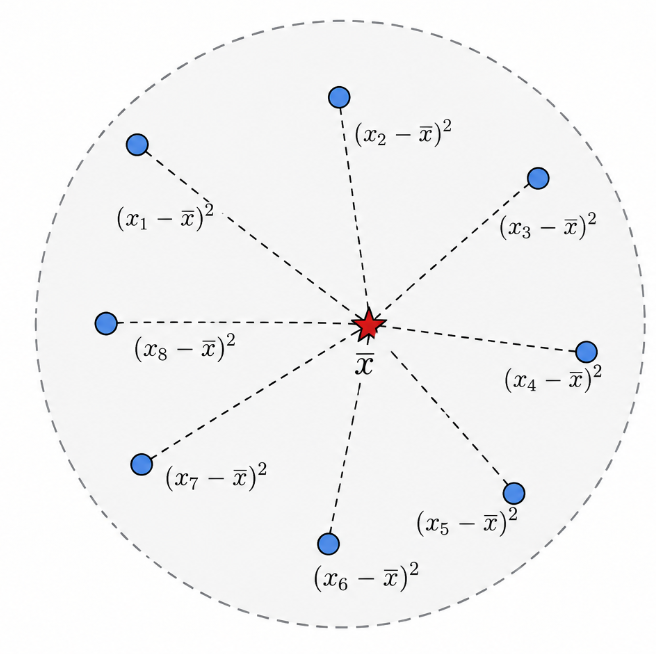
\includegraphics[width=0.7\textwidth]{figuras/variancia.png}
    \caption{Representação geométrica da variância como a média dos quadrados das distâncias das observações em relação à média.}
    \label{fig:variancia}
\end{figure}

O termo $X-\mu$ representa o desvio de $X$ em relação à sua média. Entretanto, simplesmente calcular a média desses desvios não seria útil, pois desvios positivos e negativos poderiam se cancelar. Por esse motivo, consideramos o quadrado dos desvios.

Como
\begin{equation*}
    (X-\mu)^2\geq0,
\end{equation*}
temos necessariamente
\begin{equation*}
    \operatorname{Var}(X)\geq0.
\end{equation*}

Quanto menor a variância, mais concentrados tendem a estar os valores de $X$ em torno de sua esperança. Quanto maior a variância, maior tende a ser a dispersão desses valores.

Uma forma bastante útil para o cálculo da variância é
\begin{equation*}
    \operatorname{Var}(X) =\mathbb{E}[X^2]-\left(\mathbb{E}[X]\right)^2.
\end{equation*}

Essa expressão é equivalente à definição anterior e, em muitos problemas, simplifica consideravelmente os cálculos.


\begin{defin}
    Se $X$ é uma variável aleatória discreta com função de probabilidade $p(x)=\mathbb P(X=x)$ e média $\mu=\mathbb{E}[X]$, então
\begin{equation*}
    \operatorname{Var}(X)=\sum_x (x-\mu)^2\mathbb P(X=x).
\end{equation*}

Equivalentemente, podemos utilizar
\begin{equation}
    \operatorname{Var}(X) =\sum_x x^2\mathbb P(X=x)-\mu^2.
\end{equation}

\end{defin}

Portanto, para calcular a variância de uma variável aleatória discreta, podemos primeiramente determinar $\mathbb{E}[X]$ e $\mathbb{E}[X^2]$ e, posteriormente, utilizar
\begin{equation}
\operatorname{Var}(X) =\mathbb{E}[X^2]-\left(\mathbb{E}[X]\right)^2\,\,\footnote{Esta expressão vale tanto para caso discreto quanto contínuo, mudando assim apenas a forma com que se calcula as esperanças}
\end{equation}

Se $X$ é uma variável aleatória contínua com função densidade $f_X(x)$ e média $\mu=\mathbb{E}[X]$, então
\begin{equation*}
    \operatorname{Var}(X) =\int_{-\infty}^{+\infty}(x-\mu)^2f_X(x),dx.
\end{equation*}

\begin{equation*}
    \mathbb{E}[X^2] =\int_{-\infty}^{+\infty}x^2f_X(x),dx.
\end{equation*}

Assim, embora as expressões utilizadas nos casos discreto e contínuo sejam diferentes, a ideia por trás da variância é exatamente a mesma: medir o grau de dispersão dos possíveis valores da variável aleatória em torno de sua esperança.

De maneira resumida,
\begin{equation*}
\operatorname{Var}(X)
=\begin{cases}
\displaystyle\sum_x (x-\mu)^2\mathbb P(X=x), & \text{se $X$ é discreta},\\
\displaystyle\int_{-\infty}^{+\infty}(x-\mu)^2f_X(x),dx, & \text{se $X$ é contínua}.
\end{cases}
\end{equation*}

\section{Correlação entre Variáveis}

A correlação é uma medida utilizada para quantificar a intensidade e a direção da relação linear entre duas variáveis aleatórias. Antes de defini-la formalmente, é conveniente introduzir a \textbf{covariância}. Sejam $X$ e $Y$ duas variáveis aleatórias com esperanças finitas. A covariância entre $X$ e $Y$ é definida por
\begin{equation}
\label{correlacao}
    \operatorname{Cov}(X,Y)=\mathbb{E}\left[(X-\mathbb{E}[X])(Y-\mathbb{E}[Y])\right].
\end{equation}

Equivalentemente, podemos escrever a equação~\ref{correlacao} como 

$$\operatorname{Cov}(X,Y)=\mathbb{E}[XY]-\mathbb{E}[X]\mathbb{E}[Y]\quad \footnote{Essa expressão deriva do desenvolvimento dos produtos dentro da definição e utilização de propriedades de esperança. }$$ 

    Intuitivamente, a covariância indica como $X$ e $Y$ tendem a variar conjuntamente. Quando $\operatorname{Cov}(X,Y)>0$, valores de $X$ acima de sua média tendem a estar associados a valores de $Y$ também acima de sua média. Quando $\operatorname{Cov}(X,Y)<0$, ocorre o comportamento oposto: valores elevados de uma variável tendem a estar associados a valores menores da outra.

Entretanto, a magnitude da covariância depende das unidades de medida de $X$ e $Y$, dificultando a comparação entre diferentes pares de variáveis. Para eliminar essa dependência de escala, utilizamos o \textbf{coeficiente de correlação de Pearson}, definido, para $\operatorname{Var}(X)>0$ e $\operatorname{Var}(Y)>0$, por
\begin{equation}
    \rho_{X,Y}=\frac{\operatorname{Cov}(X,Y)}{\sqrt{\operatorname{Var}(X)\operatorname{Var}(Y)}}.
\end{equation}

O coeficiente de correlação satisfaz $-1\leq\rho_{X,Y}\leq1$. Valores de $\rho_{X,Y}$ próximos de $1$ indicam uma forte associação linear positiva, enquanto valores próximos de $-1$ indicam uma forte associação linear negativa. Por outro lado, valores próximos de zero indicam ausência, ou baixa intensidade, de uma relação \textbf{linear} entre as variáveis.

\begin{figure}[h]
    \centering
    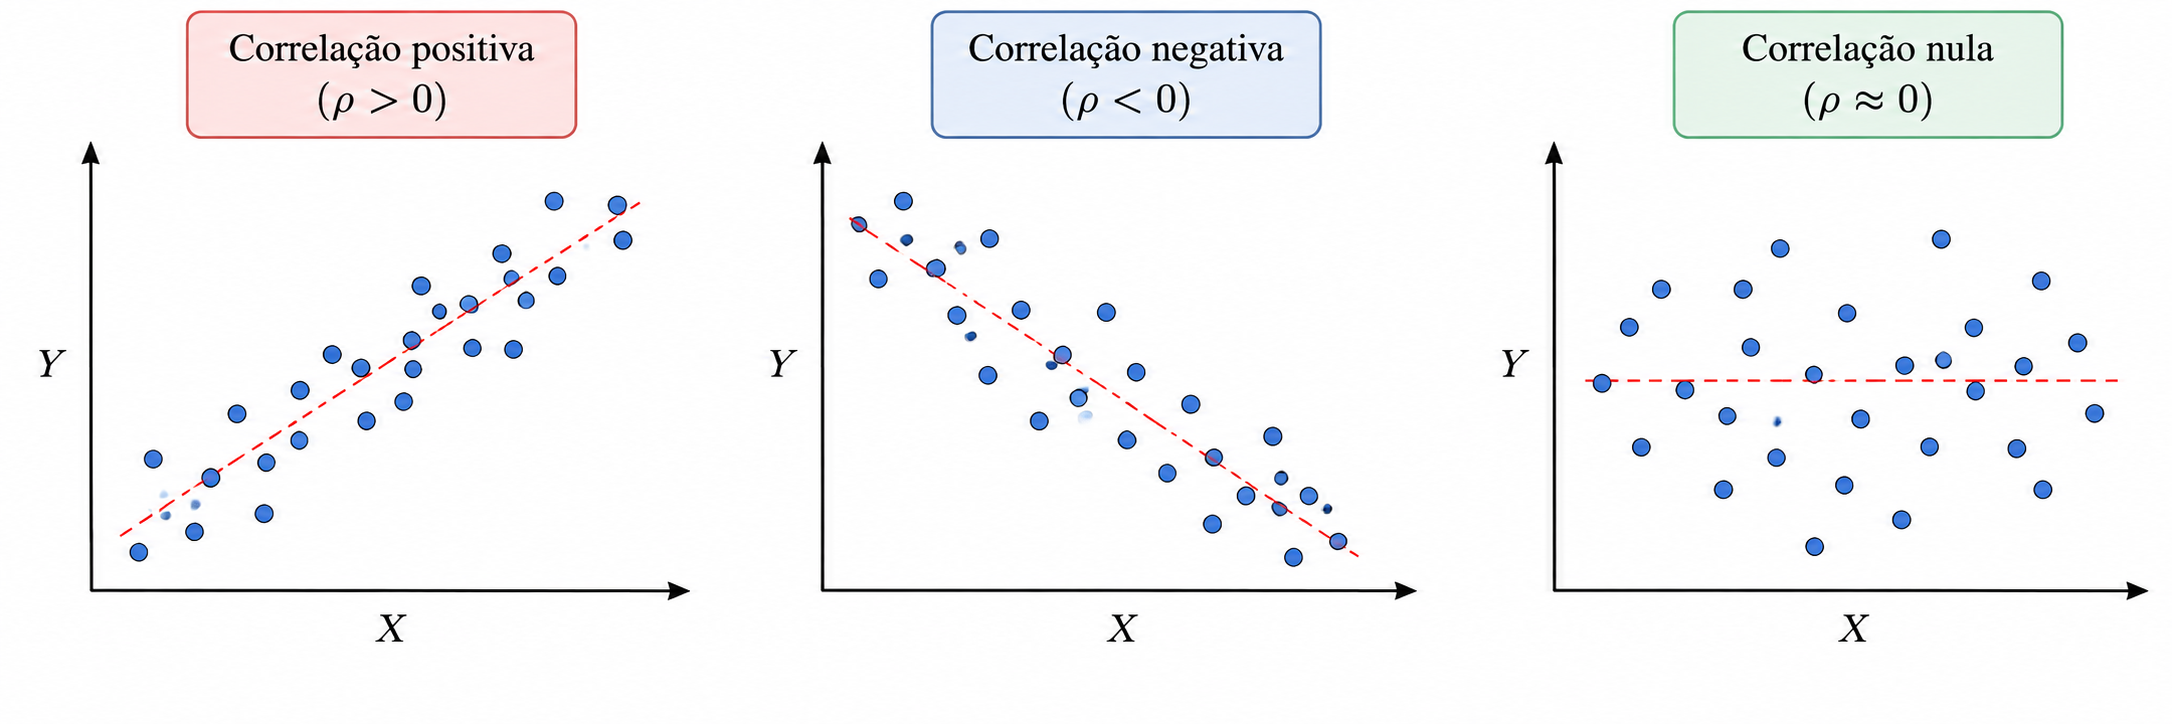
\includegraphics[width=.8\textwidth]{figuras/correlacao.png}
    \caption{Representação gráfica de diferentes padrões de correlação entre duas variáveis aleatórias $X$ e $Y$: correlação positiva, correlação negativa e ausência de correlação linear.}
    \label{fig:correlacao}
\end{figure}

É importante destacar que $\rho_{X,Y}=0$ não significa, em geral, que $X$ e $Y$ sejam independentes. Variáveis podem possuir uma forte relação não linear e, ainda assim, apresentar correlação igual a zero. Por outro lado, se $X$ e $Y$ são independentes e possuem segundos momentos finitos, então $\operatorname{Cov}(X,Y)=0$ e, consequentemente, $\rho_{X,Y}=0$, desde que ambas possuam variâncias positivas. Portanto, a correlação deve ser interpretada especificamente como uma medida de \textbf{associação linear}, e não como uma medida geral de dependência entre variáveis aleatórias.

\exercicios

    \item Considere uma sequência de lançamentos independentes de uma moeda honesta e de um dado honesto. Para $i=1,\ldots,N$, defina
\begin{equation*}
    X_i=
    \begin{cases}
        1, & \text{se a moeda resultar em cara},\\
        0, & \text{se a moeda resultar em coroa},
    \end{cases}
    \qquad
    Y_i=
    \begin{cases}
        -1, & \text{se o resultado do dado for par},\\
        1, & \text{se o resultado do dado for ímpar}.
    \end{cases}
\end{equation*}
Suponha ainda que os lançamentos da moeda e do dado sejam independentes e, para $m\leq N$, considere a variável aleatória
\begin{equation*}
    Z^{(m)}=\sum_{i=1}^{m}X_iY_i.
\end{equation*}
\begin{enumerate}
    \item[(a)] Determine a distribuição de $Z^{(m)}$.
    \item[(b)] Calcule $\mathbb E\left[Z^{(m)}\right]$ e $\operatorname{Var}\left(Z^{(m)}\right)$.
    \item[(c)] Determine $\mathbb P\left(Z^{(m)}=0\right)$ em função de $m$.
\end{enumerate}

\fimexercicios







 

 
	
	
	
	
	
\bibliographystyle{ieeetr} % plain abbrv newapa apa apalike plainnat amsplain abbrvnat unsrtnat ieeetr
\bibliography{bibliografia}
%\printbibliography 

\end{document}
